\documentclass[11pt,]{article}
\usepackage{lmodern}
\usepackage{amssymb,amsmath}
\usepackage{ifxetex,ifluatex}
\usepackage{fixltx2e} % provides \textsubscript
\ifnum 0\ifxetex 1\fi\ifluatex 1\fi=0 % if pdftex
  \usepackage[T1]{fontenc}
  \usepackage[utf8]{inputenc}
\else % if luatex or xelatex
  \ifxetex
    \usepackage{mathspec}
  \else
    \usepackage{fontspec}
  \fi
  \defaultfontfeatures{Ligatures=TeX,Scale=MatchLowercase}
\fi
% use upquote if available, for straight quotes in verbatim environments
\IfFileExists{upquote.sty}{\usepackage{upquote}}{}
% use microtype if available
\IfFileExists{microtype.sty}{%
\usepackage{microtype}
\UseMicrotypeSet[protrusion]{basicmath} % disable protrusion for tt fonts
}{}
\usepackage[margin=1in]{geometry}
\usepackage{hyperref}
\hypersetup{unicode=true,
            pdftitle={Etude des effets des pésticides dans la production des vins de table},
            pdfauthor={A. Blanc, N. Gusarov, S. Picon},
            pdfborder={0 0 0},
            breaklinks=true}
\urlstyle{same}  % don't use monospace font for urls
\usepackage{longtable,booktabs}
\usepackage{graphicx,grffile}
\makeatletter
\def\maxwidth{\ifdim\Gin@nat@width>\linewidth\linewidth\else\Gin@nat@width\fi}
\def\maxheight{\ifdim\Gin@nat@height>\textheight\textheight\else\Gin@nat@height\fi}
\makeatother
% Scale images if necessary, so that they will not overflow the page
% margins by default, and it is still possible to overwrite the defaults
% using explicit options in \includegraphics[width, height, ...]{}
\setkeys{Gin}{width=\maxwidth,height=\maxheight,keepaspectratio}
\IfFileExists{parskip.sty}{%
\usepackage{parskip}
}{% else
\setlength{\parindent}{0pt}
\setlength{\parskip}{6pt plus 2pt minus 1pt}
}
\setlength{\emergencystretch}{3em}  % prevent overfull lines
\providecommand{\tightlist}{%
  \setlength{\itemsep}{0pt}\setlength{\parskip}{0pt}}
\setcounter{secnumdepth}{5}
% Redefines (sub)paragraphs to behave more like sections
\ifx\paragraph\undefined\else
\let\oldparagraph\paragraph
\renewcommand{\paragraph}[1]{\oldparagraph{#1}\mbox{}}
\fi
\ifx\subparagraph\undefined\else
\let\oldsubparagraph\subparagraph
\renewcommand{\subparagraph}[1]{\oldsubparagraph{#1}\mbox{}}
\fi

%%% Use protect on footnotes to avoid problems with footnotes in titles
\let\rmarkdownfootnote\footnote%
\def\footnote{\protect\rmarkdownfootnote}

%%% Change title format to be more compact
\usepackage{titling}

% Create subtitle command for use in maketitle
\providecommand{\subtitle}[1]{
  \posttitle{
    \begin{center}\large#1\end{center}
    }
}

\setlength{\droptitle}{-2em}

  \title{Etude des effets des pésticides dans la production des vins de table}
    \pretitle{\vspace{\droptitle}\centering\huge}
  \posttitle{\par}
  \subtitle{Analyse empirique des marchés}
  \author{A. Blanc, N. Gusarov, S. Picon}
    \preauthor{\centering\large\emph}
  \postauthor{\par}
      \predate{\centering\large\emph}
  \postdate{\par}
    \date{19/12/2019}

\usepackage{array}
\usepackage{multicol}
\usepackage{graphicx}
\usepackage{placeins}

\begin{document}
\maketitle

\hypertarget{introduction}{%
\section{Introduction}\label{introduction}}

\textbf{Quel est l'effet de l'utilisation des pesticides sur le marché des vins simples ?}

Dans cette étude, nous chercherons à étudier l'équilibre sur le marché
du vin.

\hypertarget{les-pesticides}{%
\section{Les pesticides}\label{les-pesticides}}

\begin{itemize}
\tightlist
\item
  Présentation du problème des pésticides
\item
  Etat actuel
\item
  Comment baisser l'utilisation de pesticides
\end{itemize}

\hypertarget{presentation-du-probleme-des-pesticides}{%
\subsection{Présentation du problème des
pesticides}\label{presentation-du-probleme-des-pesticides}}

\begin{itemize}
\tightlist
\item
  Source de nombreux débats sur la santé et l'environnement.
\item
  Le rôle actuel :

  \begin{itemize}
  \tightlist
  \item
    Moyen de protection contre les aléas climatiques ;
  \item
    Outil pour la réservation du rendement.
  \end{itemize}
\item
  Plusieurs mesures mises en places pour réduire leurs usages :

  \begin{itemize}
  \tightlist
  \item
    des interdiction des produits les plus toxiques ;
  \item
    l'instauration d'une taxe, payée par les agriculteurs (Butault et
    al, 2011).
  \end{itemize}
\item
  Malgres les efforts l'utilisation perdure :

  \begin{itemize}
  \tightlist
  \item
    Hausse des ventes de produits phytosanitaires ;
  \item
    Augmentation des doses utilisés (+12\% en 2014-2016) ;
  \end{itemize}
\end{itemize}

\hypertarget{etat-actuel}{%
\subsection{Etat actuel}\label{etat-actuel}}

Contrairement aux attentes des autorités aucune baisse de l'utilisation
de pesticides :

\begin{itemize}
\tightlist
\item
  Le nombre de doses unité augmente de 23\% entre 2008 et 2017 ;
\item
  Le nombre de substances actives utilisées a augmenté de 15\% entre
  2011 et 2017 ;
\item
  Une baisse des produits les plus dangereux de 6\%, en 2017 (Moghaddam
  et al, 2019) ;
\item
  Les grandes cultures (blés, etc\ldots{}) sont les premières
  utilisatrices de pesticides 67.4\% ;
\item
  Les vignes sont les deuxièmes 14.4\% (Butault et al, 2011).
\end{itemize}

\hypertarget{comment-baisser-lutilisation-de-pesticides}{%
\subsection{Comment baisser l'utilisation de
pesticides}\label{comment-baisser-lutilisation-de-pesticides}}

Les méthodes contemporaines visant à baisser l'utilisation des
pésticides sont :

\begin{itemize}
\tightlist
\item
  Le changement de mode de culture :

  \begin{itemize}
  \tightlist
  \item
    agriculture biologique ;
  \item
    agriculture raisonnée ;
  \end{itemize}
\item
  La diversification des cultures, ce qui est impossible pour la vigne
  (Moghaddam et al, 2019).
\end{itemize}

\hypertarget{le-marche-du-vin-francais}{%
\section{Le marché du vin français}\label{le-marche-du-vin-francais}}

La France est l'un des principaux producteurs et vendeurs de vin dans le
monde. En effet, la France représente 10\% de la surface de vigne dans
le monde. La surface de vigne française se répartit dans 65 des 95
départements de la métropole. En France, il y a plus de 750000 hectares
de vignes qui sont exploitées en 2018. Ainsi, en France, une
exploitation agricole sur cinq est une exploitation viticole. Cela
représente 85000 exploitations. La production de vins en France,
représentait 4,6 milliard de litres. Cela représentait plus de 17\% de
la production totale de vin. En volume de production la France se place
donc en deuxième position derrière le volume de production de l'Italie.
3\% de la surface agricole est consacrée à la production de vin.
Néanmoins, le vin représente 15\% de la production agricole en valeur.
Du côté du consommateur, la France est le deuxième pays consommateur de
vin derrière les Etats Unis. En effet, la consommation de vin en France
représentait plus de 3,5 milliards de bouteille, en 2018. Néanmoins, on
remarque une baisse de la consommation Française depuis une trentaine
d'année.

\hypertarget{le-probleme-dheterogeneite}{%
\subsection{Le problème
d'heterogénéité}\label{le-probleme-dheterogeneite}}

Il existe une forte hétérogénéité entre les différents labels mais aussi
à l'intérieur de ces labels.

Dans le commerce du vin, il est courant de diviser les vins en deux
grandes classes en fonction de leurs prix (Cembalo et al., 2014) :

\begin{itemize}
    \item les vins de qualité inférieure, les moins chers avec les caractéristiques de qualité de base ;
    \item les vins de qualité supérieure plus chers, dotés de caractéristiques qualitatives complexes et d'une image de grande valeur.
\end{itemize} 
\par

De plus, pour les vins français, selon Steiner (2014), le système
européen de classification des
``\textit{vins de qualité produits dans certaines régions}'' (VQPRD)
contient à la fois des vins AOC et des
``\textit{vins de haute qualité provenant d'un vignoble régional agréé}''
(VDQS). Les vins de cépage appartiennent à la catégorie des vins autres
que VQPRD, qui comprend les \textbf{vins de table} et les
\textbf{vins de pays}.

\par

En tenant compte des spécificités du marhcé du vin français, nous
utilisons la méthodologie du ministère d'agriculture et divisons le
marché en deux parties :

\begin{itemize}
    \item La gamme haute (les vins IGP, vendus dans des magasins spécifiques) ;
    \item La gamme basse (les vins non IGP, vendus en grands surfaces).
\end{itemize}
\par

La première partie est soumise à des règlements spécifiques :
limitations des quantités produites, origine contrôlé, un caractère de
la demande spécifique. La deuxième, c'est-à-dire le marché des vins
moins chers, est aussi complexe. Les produits classés dans cette
catégorie sont susceptibles d'avoir un certain degré d'hétérogénéité,
comme cela a été montré par Cembalo et al.~(2014).

\par

\hypertarget{les-vins-de-table}{%
\subsection{Les vins de table}\label{les-vins-de-table}}

Ces vins sans indication géographique (sans IG) ont vu leurs
transactions augmenter en volume pour toutes les couleurs. Ainsi, on
remarque que pour les vins rouges les transactions ont augmenté de 10\%,
pour les rosées la hausse représentait 52\%, pour les vins blancs les
volumes de transactions ont presque été doublé. Néanmoins on remarque
une baisse des cours des vins sans indication géographique. En effet, on
remarque que les prix moyens pour les vins rouges et rosées sans
indication géographique baisse de 3\%. Le prix moyen des vins blancs
baisse quand à eux de 12\%, pour la campagne 2019/2020. Sur les deux
mois de campagne, les échanges de Vin sans indication géographique est
de 142 milliers d'hectolitres. Cela correspond à une hausse de 39\% par
rapport à la campagne précédente. Les ventes représentent 92 milliers
d'hectolitres. La tendance sur le marché des vins sans indication
géographique s'explique par une forte hausse des vins blancs. En effet,
ceux-ci connaissent une hausse de près de 28 milliers d'hectolitres,
soit une hausse de 232\% vis-à-vis de la campagne de 2018-2019. Les vins
rosés connaissent également une hausse. Néanmoins, celle-ci reste
modeste puisque les ventes augmentaient de 61\% par rapport à la
campagne 2018/2019. Néanmoins, les ventes de vins rouges ont légèrement
baissé. Le cours des Vins sans indication géographique baisse par
rapport à la campagne précédente.

\par

Lors de la campagne 2018/2019, les ventes de vins en grande distribution
sont en baisse. Cela peut s'expliquer par une hausse des prix moyens.
Les ventes de vins représentent 8,7 millions d'hectolitres et un chiffre
d'affaires de 4,1 milliards d'euros avec un prix moyen de 4,73
euro/litre. La baisse de la consommation de vins rouges s'aggrave avec
une baisse de 8\% par rapport à la campagne de 2017/2018. Les vins
blancs connaissent aussi une faible baisse de 1,2\% en volume par
rapport à la consommation de la campagne précédente. Pour finir, les
ventes de vins rosés ont baissé lors de la campagne 2018/2019. En effet,
on enregistre une baisse de 3,9\% en volume par rapport à la campagne
2017/2018. La consommation de vin sans indication géographique est de
6\% en volume contre 3\% en valeur. Les ventes de vins sans indications
géographiques sont en légère hausse dans la campagne 2018/2019 par
rapport à la campagne 2017/2018.

\par

Dans notre étude, nous traitons uniquement les vins simples (non IGP).
La situation sur ce marché est sensée influencer l'utilisation des
pesticides, car les volumes de productions sont plus significatives que
pour le marché des vins IGP.

\par

Suivant le raisonnement des chercheurs Cembalo et al.~(2014), dans une
catégorie de vin avec une fourchette de prix étroite, il existe une
homogénéité presque parfaite due à des vins ayant des attributs
intrinsèques simples, une complexité de qualité médiocre et donc une
différenciation peu marquée.

\par

Cela nous permet d'analyser le marché par département est non par des
marques/produits.

\hypertarget{utilisation-des-pesticides-dans-la-viticulture}{%
\subsection{Utilisation des pesticides dans la
viticulture}\label{utilisation-des-pesticides-dans-la-viticulture}}

Les phytosanitaires sont très utilisés dans les cultures comme la
viticulture. Il s'agit donc d'un intrant important pour la production de
vin. Ainsi, la viticulture utilisait 15\% de produit phytosanitaire. La
pression sanitaire varie selon les productions. Elle est forte en
viticulture. De la même façon, la pression phytosanitaire varie selon
les régions. Ainsi, pour la vigne l'IFT varie de 7 en Provence à 22 en
Champagne.

\hypertarget{le-modele-theorique}{%
\section{Le Modèle théorique}\label{le-modele-theorique}}

\hypertarget{les-hypotheses-theoriques}{%
\subsection{Les hypothèses théoriques}\label{les-hypotheses-theoriques}}

Comme proposé dans la littérature, notre étude sur les vins non coûteux
(non IGP) est effectué au niveau du pays Cembalo et al.~(2014) pour deux
raisons :

\begin{itemize}
    \item Les prix de vente moyens des marchés sont diffèrent en raison des droits de douane à l'importation et des taxes à la consommation différents % (Anderson et Nelgen 2011);
    \item La perception des produits de consommation varie d'un pays à l'autre % (Makela et al. 2006).
\end{itemize}
\par

La plupart des bouteilles achetées sont achetées dans la grande
distribution. Néanmoins, dans un souci de simplicité nous estimerons que
les consommateurs achètent leurs bouteilles directement auprès du
viticulteur. Donc nous supprimerons tous les intermédiaires entre le
producteur et le marché final.

\par

Quand aux exportations et les importations, n'ayant pas la possibilité
contrôler le montant des vins non IGP exportés/importés, nous laissons
ces effets au terme d'erreur. Nous ignorons les interactions
internationales completement.

\par

Pour conclure, nos suppositions au niveau du marché des vins sont les
suivantes :

\begin{itemize}
    \item La demande pour les vins simples est unique pour toute la France. On n'observe pas les quantités consommés par départements, mais pour tout le pays, avec un prix unique. 
    \item La production du vin varie par département, suite à des différences climatologiques.
    \item On n'observe que l'équilibre sur le marché au niveau du pays (la quantité demandé est égale à la quantité offerte par l'ensemble des régions).
\end{itemize}
\par

En ce qui concerne les pesticides, nous supposons que :

\begin{itemize}
    \item La demande des pesticides est inélastique au prix, ce qui nous permet d'exclure la partie de l'offre des pesticides du notre analyse. La quantité de pesticides utilisée demande seulement des intentions et des besoins des agriculteurs. 
\end{itemize}

\hypertarget{formalisation}{%
\subsection{Formalisation}\label{formalisation}}

En formalisant notre modèle théorique, nous posons, que la demande de
vin a la forme suivante : \begin{equation}
    Q_d = \alpha_d + \beta_d P_d + \gamma_d Z 
\end{equation} Avec \(Z\) étant l'ensemble des variables ayant une
influence sur la demande du vin, dans le cas le plus simple nous
n'utilisons que les revenus (c'est une des variables les plus utilisées
dans des études empiriques sur le marché du vin).

\par

L'offre totale pour toute la France est donnée par l'équation suivante :
\begin{equation}
    Q_o = \sum_{i = 1}^{N} q_i
\end{equation} Ou \(i \in \{1, ..., N\}\) sont des départements, chacun
ayant sa propre fonction de production et d'offre unique :
\begin{equation}
    q_i = a_i + b_i P_o + c_i X
\end{equation} Avec \(X\) étant un vecteur des variables explicatives
influençant la production (dans le cas le plus simple nous ne prenons en
compte que les quantités des pesticides utilisées). Nous pouvons
réécrire l'équation de l'offre sous la forme : \begin{equation}
    Q_o = \sum_{i = 1}^{N} (a_i + b_i P_o + c_i X) = \sum_{i = 1}^{N} a_i + \sum_{i = 1}^{N} b_i P_o + \sum_{i = 1}^{N} c_i X
\end{equation} Nous obtenons enfin un système de \(N + 2\) équations :
\begin{align*}
    Q_d & = \alpha_d + \beta_d P_d + \gamma_d Z \\
    Q_o & = \sum_{i = 1}^{N} q_i \\
    q_{1,t} & = a_1 + b_1 P_o + c_1 X \\ 
    \vdots \\ 
    q_{N,t} & = a_N + b_N P_o + c_N X \\
\end{align*} Quand même, parce que nous pouvons supposer une presence
des contraintes au niveau des données, nous devrions prévoir des
modifications possibles pour notre modèle. Les contraintes principales
sont au niveau du manque des données au niveau des années, c'est-à-dire
que nous risquons d'avoir une trés faibles variation intra-annuelle des
prix et de revenus pour pouvoir identifier les coefficient associés par
un passage à l'équation structurelle.

\par

Une de ces modification possibles est l'introduction d'une contrainte
supplementaire au niveau de la demande sur le vin de table. Afin de
pouvoir identifier les effets de toutes les variables par un système
AIDS, nous pouvons supposer, que tout le vin produit dans un département
est consommé dans le même department. C'est une hypothèse forte, qui
nous éloigne de la réalité, parce que de cette façon nous ignorons
plusieurs effets pervers, tels que :

\begin{itemize}
  \item La structure du marché interne de la France ;
  \item La mobilité de la production entre les differents départements ;
  \item L'export du vin ;
  \item La consommation des vins importés.
\end{itemize}
\par

Nous pouvons tout de méme ignorer ces effets, car nous visons à estimer
les effets moyens pour tous les départements. De cette façon lors
d'aggregation des effets au niveau national nous allons mitiger les
biais possibles.

\par

Alors,nous pouvons réécrire notre système d'equations sous la forme
suivante : \begin{align*}
  qd_1 & = \alpha_{1} + \beta P_{1,d} + \gamma_{1} Z_{1} \\
  \vdots \\ 
  qd_N & = \alpha_{N} + \beta P_{N,d} + \gamma_{N} Z_{N} \\
  qo_1 & = a_1 + b P_{1,o} + c_1 X_{1} \\ 
  \vdots \\ 
  qo_N & = a_N + b P_{N,o} + c_N X_{N} \\
\end{align*} Il faut specifier, que nous supposons les effets de prix
sont identiques pour tous les département en moyenne, tandis que nous
laissons quand même les effets des autres variables dépéndantes (ex : le
revenu et les pésticides) de varier par département.

\hypertarget{les-donnees}{%
\section{Les données}\label{les-donnees}}

\hypertarget{sources-des-donnees}{%
\subsection{Sources des données :}\label{sources-des-donnees}}

Nous avons utilisé les bases des données suivantes pour notre analyse :

\begin{itemize}
    \item Les données de ventes de pesticides par département  (INERIS)
    \item Les données sur les prix du vin (France Agrimer)
    \item Les données sur la population (INSEE)
    \item Les données sur la production de vin (SSM Finances Publiques)
\end{itemize}
\par

\hypertarget{les-variables-utilisees-pour-notre-modele}{%
\subsection{Les variables utilisées pour notre
modèle}\label{les-variables-utilisees-pour-notre-modele}}

Dans notre étude nous faisons face à un problème avec deux variables
endogènes et trois variables exogènes.

\begin{itemize}
\tightlist
\item
  Variables endogènes :

  \begin{itemize}
  \tightlist
  \item
    la quantité totale produite de vin rouge et blanc non IG par
    département (en hectolitres, en log),
  \item
    le prix moyen des vins rouges-blancs (idice, en log).
  \end{itemize}
\item
  Variables exogènes :

  \begin{itemize}
  \tightlist
  \item
    le revenu médian par département (en euros par personne par année,
    en log),
  \item
    la surface agricole destinée aux vins de table (en hectares, en
    log),
  \item
    la quantité des pesticides utilisés sur la vigne (indice, en log).
  \end{itemize}
\end{itemize}

Au niveau des pesticides, on va s'intéresser plus particulièrement aux
quantités de produits vendus par département entre 2009 et 2017 utilisés
principalement sur les cultures viticoles. Il faut faire preuve de
vigilance sur le conditionnement des produits qui n'est pas exprimé dans
la même unité au sein de cette base : en litres ou en kilos. Dans notre
étude nous allons étudier l'impact de la masse totale des pésticides
utilisés. Pour pouvoir le faire, nous créons un indice qui permet de
prendre en compte les évolutions des differents types des produits à la
fois. Nous créons un indice simple : \begin{equation*}
  P = \frac{\sum_j p_{j, t} q_{j, t}}{\sum_j p_{j, 0} q_{j, 0}}
\end{equation*} Avec \(j\) désignant le produit \(j\), et \(p\) étant un
coefficient de pondération (dans le cas le plus simple \(p = 1\)).

\par

En ce qui concerne les données sur le prix du vin, on s'intéresse
principalement au prix moyen des vins rouge- rosés et blancs sans IG
(Indication Géographique) sur la période 2009-2017. Ces prix sont
déflatés par l'indice des prix à la consommation (base 100 en 2014). On
ne considère ici que le prix moyen déflaté au niveau national. Dans le
deuxième modèle nous avons besoin de créer artificiellement un
estimateur qui va varier par département. Dans ce but nous créons
l'indice de prix du vin de table départementale, calculé de façon
suivante : \begin{equation*}
  P = \frac{p_{rouge, t} q_{rouge, t} + p_{blanc, t} q_{blanc, t}}{p_{rouge, 0} q_{rouge, 0} + p_{blanc, 0} q_{blanc, 0}}
\end{equation*} Avec \(t\) étant l'anée au temps \(t\).

\par

Au niveau des données sur la population, la variable qui nous intéresse
ici est relative au niveau de revenu, exprimée au niveau départemental
(laquelle, si besoin nous pourrions facilement aggréger au niceau
national). Plus précisément, on va utiliser le revenu médian par
département. Il est aussi déflatée de l'indice des prix à la
consommation (base 100 en 2014).

\par

Enfin, nous avons exploité les variables suivantes au niveau de la
production de vin : la surface totale de culture viticole en hectares,
la surface utilisé pour les vins non IG, la quantité produite de vins
rouges-rosés et blancs sans IG en hectolitres, pour chaque département
et sur la période 2009-2017. Afin d'obtenir un estimateur de la quantité
de vin totale on prend la somme totale des tous types du vin sans IG.

\hypertarget{dictionnaire-des-variables}{%
\subsection{Dictionnaire des
variables}\label{dictionnaire-des-variables}}

\FloatBarrier

\begin{table}[!htbp]
  \centering
\caption{Ditionnaire des varibales}
\begin{tabular}{c|l}
  \hline
  Variable & Description \\
  \hline
année & année \\
ndep & numéro de département \\
si & superficie de vigne sans indication géographique en hectare en log \\
qi & quantité de vins produits en hectolitre en log \\
ipi & indice des prix du vin sans IG déflatés en log  \\
ri & revenu disponible brut des ménages français déflatés en log \\
iki & indice de quantité de pesticides achetés en log \\
t & la tendance temporelle \\
\hline
\end{tabular}
\end{table}

\FloatBarrier

Les propriétés de ces données sont suivantes :

\begin{itemize}
  \item Toutes les variables varient par département et par année.
  \item Le période temporelle comprise dans notre échantillon est de 2012 à 2016.
  \item Nous ne considérons que les régions produisant du vin. 
  \item Nous éliminons les effets fixes pour en substrayant les moyennes départamentales.
  \item Données en panel "cylindrées".
  \item Nombre des individus large (69 départements, qui produisent le vin et utilisent des pésticides) et le nombre des périodes pauvre (5 périodes).
\end{itemize}

\hypertarget{letude-statistique}{%
\section{L'étude statistique}\label{letude-statistique}}

Dans cette partie de travail nous allons explorer les données
collectées.

\par

De l'étude de la variance pour les données en panel avec des
statistiques générales, nous passerons vers l'étude des interdependances
des variables. Pui, nous allons finir avec étude des donnée alternées
par une transformation \textbf{Within}.

\hypertarget{visualisation-au-niveau-de-la-france}{%
\subsection{Visualisation au niveau de la
France}\label{visualisation-au-niveau-de-la-france}}

\begin{center}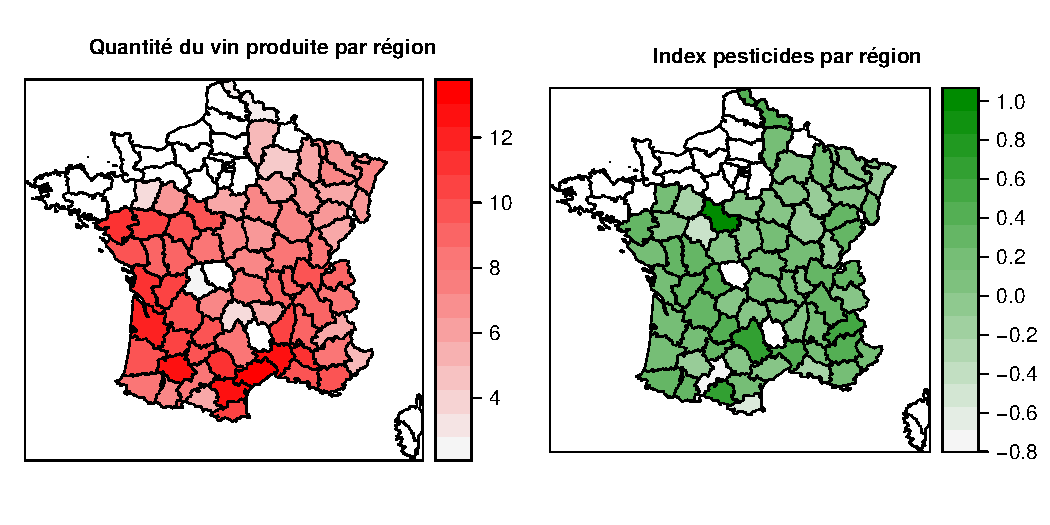
\includegraphics{note2pres_files/figure-latex/unnamed-chunk-16-1} \end{center}

\begin{center}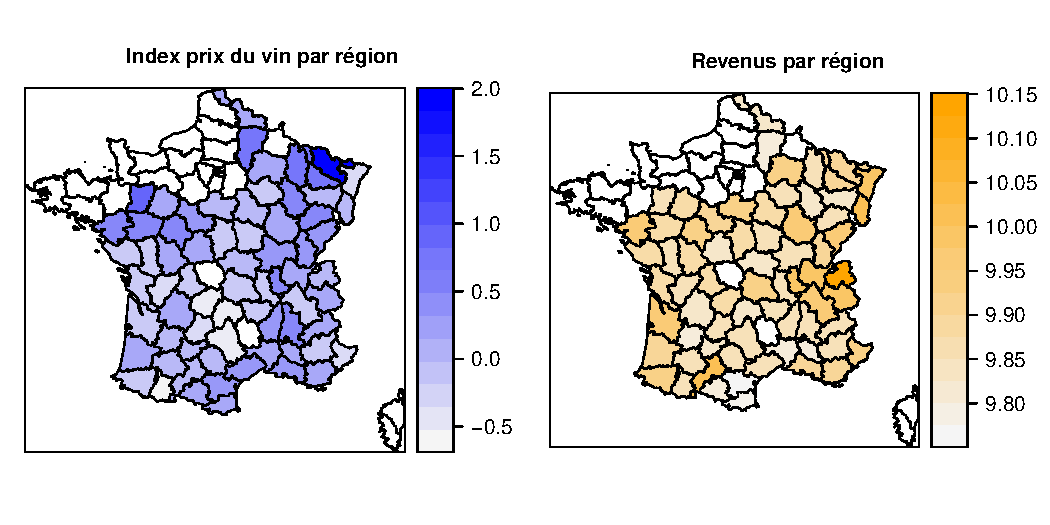
\includegraphics{note2pres_files/figure-latex/unnamed-chunk-17-1} \end{center}

\hypertarget{etude-de-la-variance}{%
\subsection{Etude de la variance}\label{etude-de-la-variance}}

Le tableau suivant regrouppe les statistiques déscriptives essentielles
:

\begin{itemize}
\tightlist
\item
  Moyennes
\item
  Variance sur l'échantillon complet
\item
  Variance \emph{between}
\item
  Variance \emph{within}
\end{itemize}

Il est facile a rémarquer que la variance \emph{between} est plus
significative que la variance \emph{within}. Cela nous amêne à l'idée
qu'il faut utiliser un modèle qui permettra estimer et corriger ces
inégalités entre les individus, car nous sommes plus interessés par des
effets individuels moyens (les effets moyens pour tous les individus).

\FloatBarrier

\begin{table}[!htbp] \centering 
  \caption{Etude de la variance} 
  \label{} 
\begin{tabular}{@{\extracolsep{5pt}} ccccc} 
\\[-1.8ex]\hline 
\hline \\[-1.8ex] 
 & Mean & Overall & Between & Within \\ 
\hline \\[-1.8ex] 
Index prix & $0.175$ & $0.568$ & $0.368$ & $0.434$ \\ 
Index pesticides & $0.170$ & $0.333$ & $0.239$ & $0.234$ \\ 
Surface & $4.892$ & $1.986$ & $1.955$ & $0.410$ \\ 
Revenus & $9.891$ & $0.061$ & $0.061$ & $0.011$ \\ 
Temps & $3$ & $1.416$ & $0$ & $1.416$ \\ 
\hline \\[-1.8ex] 
\end{tabular} 
\end{table}

\FloatBarrier

De plus, il est interessant d'observer les résultats obtenus pour le
test de Chow comparant le modèle complet (\emph{pooled model}) contre
les modèles au effet fixes et randomes.

\par

Sauf le cas de la surface nous ne pouvons pas rejeter l'hypothese nulle,
specifiant que les individus ont des effets identiques pour toute la
population.

\FloatBarrier

\begin{table}[!htbp] \centering 
  \caption{Les p-valeurs de pooling-test de Chow} 
  \label{} 
\begin{tabular}{@{\extracolsep{5pt}} ccc} 
\\[-1.8ex]\hline 
\hline \\[-1.8ex] 
 & Random & Fixed \\ 
\hline \\[-1.8ex] 
Index prix & $0.535$ & $0.533$ \\ 
Index pesticides & $0.485$ & $0.451$ \\ 
Surface & $0$ & $0.0001$ \\ 
Revenus & $0.297$ & $0.247$ \\ 
\hline \\[-1.8ex] 
\end{tabular} 
\end{table}

\FloatBarrier

\hypertarget{visualisatoin-des-interdependances}{%
\subsection{Visualisatoin des
interdependances}\label{visualisatoin-des-interdependances}}

Maintenant passons à l'étude des graphiques bivariés pour notre variable
dependante principale (la quantité du vin) et les regresseurs.

\FloatBarrier

\begin{figure}[!htbp]

{\centering 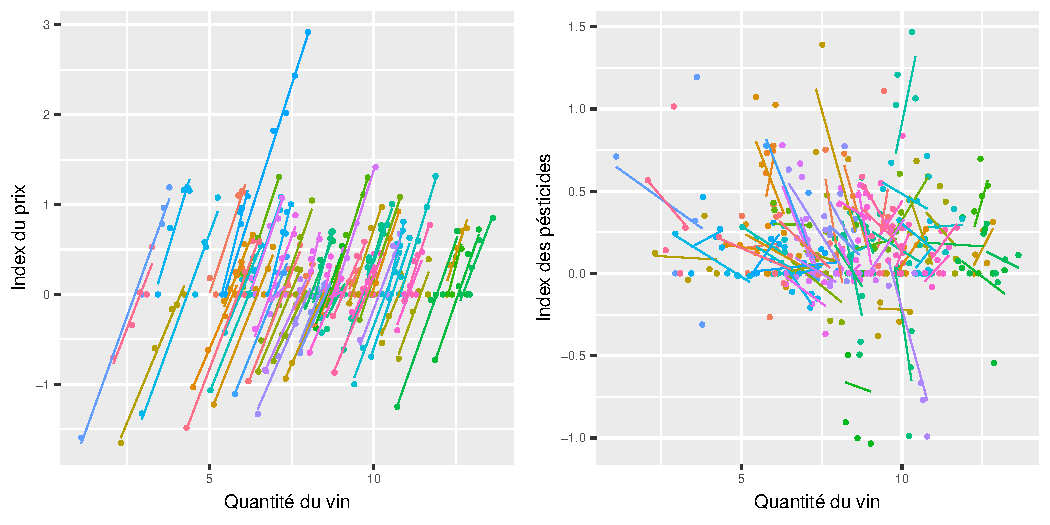
\includegraphics{note2pres_files/figure-latex/unnamed-chunk-22-1} 

}

\caption{L'étude bivarié, partie 1}\label{fig:unnamed-chunk-22}
\end{figure}

\FloatBarrier

\FloatBarrier

\begin{figure}[!htbp]

{\centering 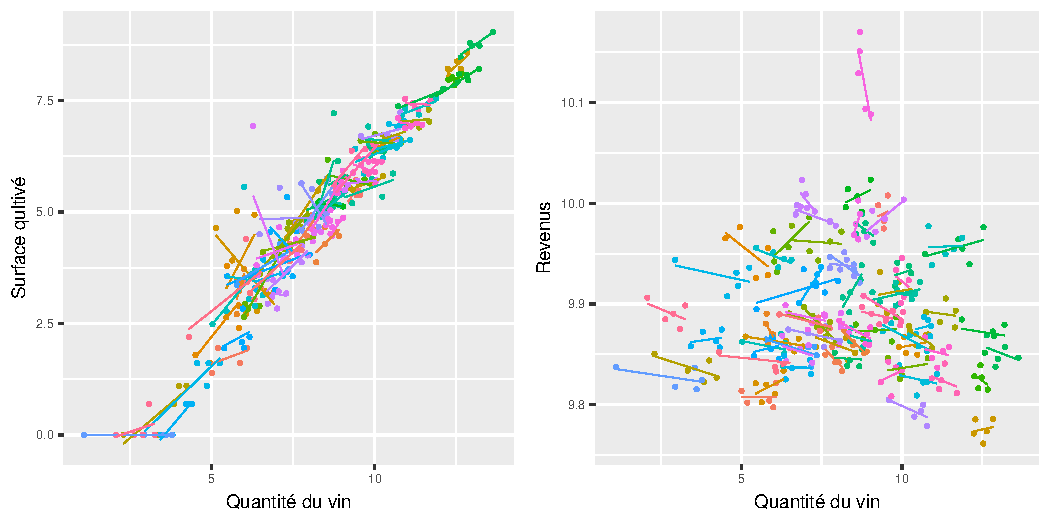
\includegraphics{note2pres_files/figure-latex/unnamed-chunk-23-1} 

}

\caption{L'étude bivarié, partie 2}\label{fig:unnamed-chunk-23}
\end{figure}

\FloatBarrier

\hypertarget{letude-des-types-deffets}{%
\subsection{L'étude des types d'effets}\label{letude-des-types-deffets}}

Nous avons déjà vu, qu'il est fortement probable que nous faisons face à
un modèle aux effets fixes individuelles. Il faut quand même le
justifier. Pour faire cela, nous allons effectuer le test de
multiplicateur de Lagrange sur la nature des effets fixes. Selon les
résultats il est évidente que nous avons des effets fixes au niveau
individuel pour toutes les variables. Pour la variable de surface nous
avons des effets à la fois individuels et temporels.

\FloatBarrier

\begin{table}[!htbp] \centering 
  \caption{p-valeurs de Lagrange multiplier test} 
  \label{} 
\begin{tabular}{@{\extracolsep{5pt}} cccc} 
\\[-1.8ex]\hline 
\hline \\[-1.8ex] 
 & Individual & Time & Twoways \\ 
\hline \\[-1.8ex] 
Index prix & $0$ & $0.169$ & $0$ \\ 
Index pesticides & $0$ & $0.222$ & $0$ \\ 
Surface & $0$ & $0.030$ & $0$ \\ 
Revenus & $0$ & $0.248$ & $0$ \\ 
\hline \\[-1.8ex] 
\end{tabular} 
\end{table}

\FloatBarrier

\hypertarget{lanalyse-de-la-correlation}{%
\subsection{L'analyse de la
correlation}\label{lanalyse-de-la-correlation}}

Maintenat nous allons comparer deux tableau de correlation. Le premier
tableau combrend les résultats pour les données telles-quelles, le
deuxieme par contre integre les résultats pour les données sous la
trasformation \emph{within}.

\FloatBarrier

\begin{longtable}[]{@{}lrrrrrr@{}}
\toprule
& Quantité du vin & IP & Surface & Revenus & Index pésticides &
Temps\tabularnewline
\midrule
\endhead
Quantité du vin & 1.0000000 & 0.1538882 & 0.9558586 & -0.0265558 &
-0.0783682 & -0.0359595\tabularnewline
IP & 0.1538882 & 1.0000000 & 0.0451726 & -0.0373917 & -0.1267030 &
0.0430476\tabularnewline
Surface & 0.9558586 & 0.0451726 & 1.0000000 & -0.0567015 & -0.0604548 &
-0.0640070\tabularnewline
Revenus & -0.0265558 & -0.0373917 & -0.0567015 & 1.0000000 & -0.0515319
& 0.1188471\tabularnewline
Index pésticides & -0.0783682 & -0.1267030 & -0.0604548 & -0.0515319 &
1.0000000 & 0.2908564\tabularnewline
Temps & -0.0359595 & 0.0430476 & -0.0640070 & 0.1188471 & 0.2908564 &
1.0000000\tabularnewline
\bottomrule
\end{longtable}

\FloatBarrier

Les rélations entre les variables mieux ressortent pour les données
transformées.

\FloatBarrier

\begin{longtable}[]{@{}lrrrrrr@{}}
\toprule
& Quantité du vin & IP & Surface & Revenus & Index pésticides &
Temps\tabularnewline
\midrule
\endhead
Quantité du vin & 1.0000000 & 0.9608421 & 0.3655017 & -0.1601237 &
-0.2275316 & -0.1994410\tabularnewline
IP & 0.9608421 & 1.0000000 & 0.2892935 & -0.0085803 & -0.1265659 &
0.0562534\tabularnewline
Surface & 0.3655017 & 0.2892935 & 1.0000000 & -0.1656929 & -0.1908549 &
-0.3103175\tabularnewline
Revenus & -0.1601237 & -0.0085803 & -0.1656929 & 1.0000000 & 0.2280372 &
0.6521815\tabularnewline
Index pésticides & -0.2275316 & -0.1265659 & -0.1908549 & 0.2280372 &
1.0000000 & 0.4139250\tabularnewline
Temps & -0.1994410 & 0.0562534 & -0.3103175 & 0.6521815 & 0.4139250 &
1.0000000\tabularnewline
\bottomrule
\end{longtable}

\FloatBarrier

\hypertarget{la-transformation-within}{%
\subsection{\texorpdfstring{La transformation
\textbf{within}}{La transformation within}}\label{la-transformation-within}}

Avant de términer cette partie d'étude statistique de notre échantillon
il faut encore présenter les rélation bivariées pour les données
transformées (sous la transformation \emph{within}).

\FloatBarrier

\begin{figure}[!htbp]

{\centering 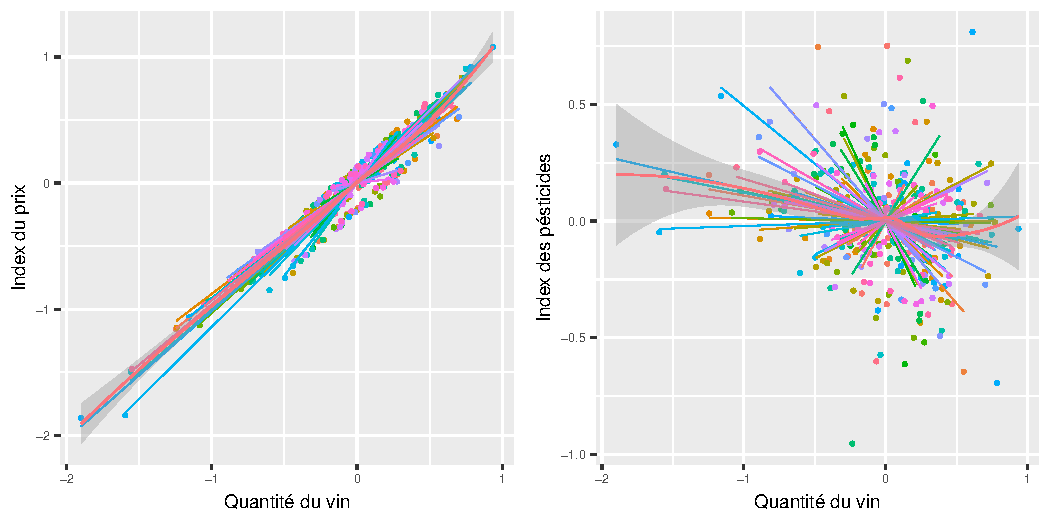
\includegraphics{note2pres_files/figure-latex/unnamed-chunk-30-1} 

}

\caption{Rélations bivariés dans le cas de transformation within, partie 1}\label{fig:unnamed-chunk-30}
\end{figure}

\FloatBarrier

\begin{figure}[!htbp]

{\centering 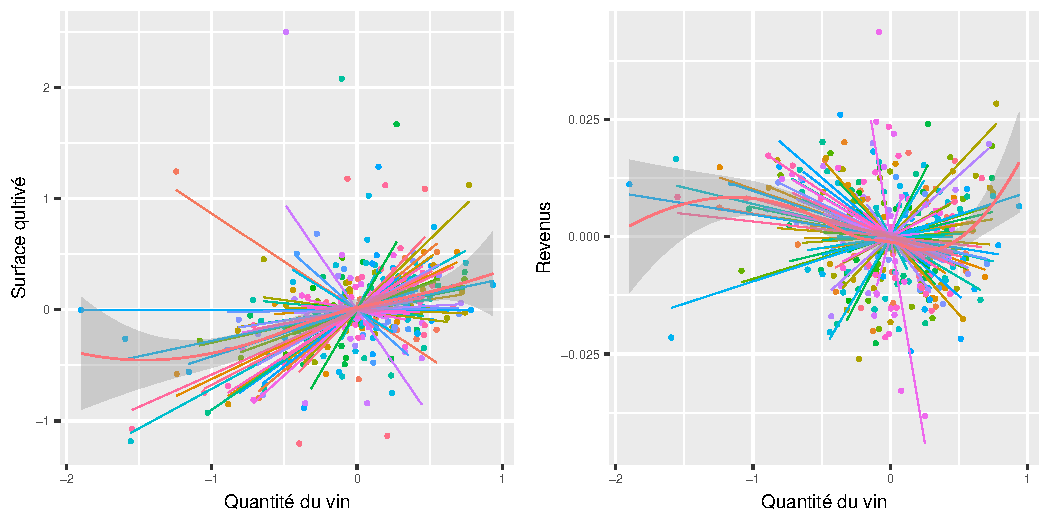
\includegraphics{note2pres_files/figure-latex/unnamed-chunk-31-1} 

}

\caption{Rélations bivariés dans le cas de transformation within, partie 2}\label{fig:unnamed-chunk-31}
\end{figure}

\FloatBarrier

\hypertarget{modelisation}{%
\section{Modèlisation}\label{modelisation}}

\begin{itemize}
\tightlist
\item
  Presentation de la méthode
\item
  Les estimations

  \begin{itemize}
  \tightlist
  \item
    OLS, WLS et SUR
  \item
    2SLS, W2SLS, 3SLS et i3SLS
  \end{itemize}
\end{itemize}

\hypertarget{presentation-de-la-methode}{%
\subsection{Presentation de la
méthode}\label{presentation-de-la-methode}}

L'AIDS et les autres modèles de demande cités dans la littérature ont de
nombreuses lacunes qui les rendent impropres pour l'estimation du marché
du vin, selon Cembalo et al.~(2014). Quand même, dans notre étude nous
allons utiliser ce modèle là, sous des suppositions restrictives.

\par

Dans cette étude, nous nous intéressons à l'effet de la quantité de
pesticides utilisé sur l'équilibre du marché des vins de table.

\hypertarget{modele-econometrique}{%
\subsection{Modèle économétrique}\label{modele-econometrique}}

Par ce modèle nous visons à estimer les effets moyenns pour tous les
départements. De cette façon lors d'aggregation des effets au niveau
national nous allons mitiger les biais possibles, liés à la
misspecification du modèle.

\par

Nous pouvons réécrire notre système d'equations sous la forme suivante :
\begin{align*}
  qd_{1,t} & = \alpha_{1} + \beta Pd_{1,t} + \gamma_{1} Z_{1,t} + \epsilon_{1,t}  \\
  \vdots \\ 
  qd_{N,t} & = \alpha_{N} + \beta Pd_{N,t} + \gamma_{N} Z_{N,t} + \epsilon_{1,t}  \\
  qo_{1,t} & = a_1 + b Po_{1,t} + c_1 X_{1,t} + u_{1,t} \\ 
  \vdots \\ 
  qo_{N,t} & = a_N + b Po_{N,t} + c_N X_{N,t} + u_{N,t} \\
\end{align*} Nous posons que l'offre et la demande sont egaux au niveau
de département. L'offre de département vise à satisfaire la demande
interne du même département. En termes d'aggregation ex-post des effets
estimés, nous sommes sensé de tomber sur l'équilibre au niveau du marché
national. C'est-à-dire : \begin{align*}
  qd_{1,t} & = qo_{1,t} \\
  \vdots \\ 
  qd_{N,t} & = qo_{N,t} \\
\end{align*} Au pint d'équilibre nous avons également l'égalité des prix
: \begin{equation*}
  Po_{1,t} = Pd_{1,t}
\end{equation*} De cette façon nous obtenons un système des systèmes des
équations : \begin{align*}
  q_{1,t} & = \alpha_{1} + \beta P_{1,t} + \gamma_{1} Z_{1,t} + \epsilon_{1,t}  \\
  \vdots \\ 
  q_{N,t} & = \alpha_{N} + \beta P_{N,t} + \gamma_{N} Z_{N,t} + \epsilon_{1,t}  \\
  q_{1,t} & = a_1 + b P_{1,t} + c_1 X_{1,t} + u_{1,t} \\ 
  \vdots \\ 
  q_{N,t} & = a_N + b P_{N,t} + c_N X_{N,t} + u_{N,t} \\
\end{align*} En simplifiant l'écriture nous pouvons la representer sous
la forme suivante : \begin{align*}
  q_{i,t} & = \alpha_{i} + \beta P_{i,t} + \gamma_{i} Z_{i,t} + \epsilon_{i,t} \\
  q_{i,t} & = a_i + b P_{i,t} + c_i X_{i,t} + u_{i,t}
\end{align*} D'ici nous avons à notre disposition deux outils
d'identification des effets étudiés :

\begin{itemize}
  \item Résolution du sytème par le passage aux équation structurelles.
  \item Doubles moindre carrés, lesquels on peut utiliser car on s'interesse principalement aux rôle de pésticides dans la production du vin ;
\end{itemize}

\hypertarget{la-srategie-didentification}{%
\subsection{La sratégie
d'identification}\label{la-srategie-didentification}}

Nous attendons à ce que l'éstimateur de 3SLS, qui permet de capter tous
les effets de correlations entre les équation en presence de plusieures
variables exogènes nous permettra d'obtenir des estimations fiables.

\begin{itemize}
\tightlist
\item
  Traitement des systèmes des équations liées (simultaneity bias)
\item
  L'estimateur de 3SLS donne des résultats similaires à l'éstimateur de
  ILS
\item
  L'estimateur est consistent
\item
  La distribuitions pour les estimateurs suit une loi normale suelement
  dans des grands échantillons
\item
  L'estimateur est efficient (asymptotiquement)
\end{itemize}

Quand même dès le debut nous envisageons des problèmes possibles avec
les résultats obtenus :

\begin{itemize}
\tightlist
\item
  Faible representation des effets hetérogenes entre les régions (nous
  estimons seulemnt les effets moyens)
\item
  Les interferences induites par l'heterogénéité
\end{itemize}

\hypertarget{resultats}{%
\section{Résultats}\label{resultats}}

Dans cette séction nous allons presenter les prémiers résultats
économétriques. Lors de ces prémiéres éstimations nous supposons que les
effets sont identiques pour tous les département (on fait la correction
pour les effets fixes au niveau départemental quand même).

\par

Nous allons presenter en particulier :

\begin{itemize}
\tightlist
\item
  Les coefficients estimés avec leurs variance
\item
  L'efficience et comparaison des estimateurs
\item
  Etude des erreurs

  \begin{itemize}
  \tightlist
  \item
    La distribution des erreurs

    \begin{itemize}
    \tightlist
    \item
      La normalité
    \item
      Centrage sur 0
    \item
      Independance des variables explicatives
    \end{itemize}
  \item
    L'autocorrelation des résidus
  \item
    L'hétéroskedacité
  \end{itemize}
\end{itemize}

Nous estimons un enseble des differents modèles afin de pouvoir choisir
la méthode la plus raisonnable. Les modèles suivantes sont traitées
séparement :

\begin{itemize}
\tightlist
\item
  Modèles simples :

  \begin{itemize}
  \tightlist
  \item
    OLS, WLS (ou nous concentrons notre attention sur l'équation d'offre
    du vin)
  \item
    SUR (ce qui n'est pas justifié, mais on l'inclus quand même)
  \end{itemize}
\item
  Modèlesdes équations simultanées avec des variables endogènes :

  \begin{itemize}
  \tightlist
  \item
    2SLS, W2SLS
  \item
    3SLS et 3SLS itérés (le dérnier modèle étant similaire à FIML)
  \end{itemize}
\end{itemize}

\hypertarget{les-resultats-ols-wls-et-sur}{%
\subsection{Les résultats OLS, WLS et
SUR}\label{les-resultats-ols-wls-et-sur}}

\FloatBarrier

\begin{table}[!htbp]
\begin{center}
\begin{tabular}{l c c c }
\hline
 & OLS & WLS & SUR \\
\hline
Demande: ipi        & $0.93^{***}$  & $0.93^{***}$  & $0.93^{***}$  \\
                    & $(0.01)$      & $(0.01)$      & $(0.01)$      \\
Demande: ri         & $-5.75^{***}$ & $-5.75^{***}$ & $-2.00^{***}$ \\
                    & $(0.47)$      & $(0.47)$      & $(0.33)$      \\
Offre: ipi          & $0.90^{***}$  & $0.90^{***}$  & $0.92^{***}$  \\
                    & $(0.01)$      & $(0.01)$      & $(0.01)$      \\
Offre: si           & $0.08^{***}$  & $0.08^{***}$  & $0.02^{*}$    \\
                    & $(0.01)$      & $(0.01)$      & $(0.01)$      \\
Offre: iki          & $-0.17^{***}$ & $-0.17^{***}$ & $-0.05^{**}$  \\
                    & $(0.02)$      & $(0.02)$      & $(0.02)$      \\
\hline
Demande: R$^2$      & 0.95          & 0.95          & 0.94          \\
Offre: R$^2$        & 0.94          & 0.94          & 0.93          \\
Demande: Adj. R$^2$ & 0.95          & 0.95          & 0.94          \\
Offre: Adj. R$^2$   & 0.94          & 0.94          & 0.93          \\
Num. obs. (total)   & 690           & 690           & 690           \\
\hline
\multicolumn{4}{l}{\scriptsize{$^{***}p<0.001$, $^{**}p<0.01$, $^*p<0.05$}}
\end{tabular}
\caption{Statistical models}
\label{table : ols, wls and sur}
\end{center}
\end{table}

\FloatBarrier

\hypertarget{independance-des-residus}{%
\subsection{Independance des résidus}\label{independance-des-residus}}

\FloatBarrier

\begin{longtable}[]{@{}lrrrrrr@{}}
\toprule
& OLS D & OLS O & WLS D & WLS O & SUR D & SUR O\tabularnewline
\midrule
\endhead
Vin & 0.2317615 & 0.2444187 & 0.2317615 & 0.2444187 & 0.2728127 &
0.2746202\tabularnewline
IP & 0.0000000 & 0.0000000 & 0.0000000 & 0.0000000 & 0.0000000 &
0.0000000\tabularnewline
Surface & 0.2707361 & 0.0000000 & 0.2707361 & 0.0000000 & 0.3131039 &
0.2364897\tabularnewline
Revenus & 0.0000000 & -0.4799169 & 0.0000000 & -0.4799169 & -0.3931430 &
-0.5421354\tabularnewline
Pesticides & -0.3082912 & 0.0000000 & -0.3082912 & 0.0000000 &
-0.3726957 & -0.2814999\tabularnewline
\bottomrule
\end{longtable}

\FloatBarrier

\hypertarget{lautocorrelation-et-lheteroskedacite}{%
\subsection{L'autocorrelation et
l'hétéroskedacité}\label{lautocorrelation-et-lheteroskedacite}}

\FloatBarrier

\begin{table}[!htbp] \centering 
  \caption{Les statistiques test de Durbin-Watson} 
  \label{} 
\begin{tabular}{@{\extracolsep{5pt}} cccc} 
\\[-1.8ex]\hline 
\hline \\[-1.8ex] 
 & OLS & WLS & SUR \\ 
\hline \\[-1.8ex] 
Equation de demande & $1.112$ & $1.112$ & $1.569$ \\ 
Equation d'offre & $1.062$ & $1.062$ & $1.552$ \\ 
\hline \\[-1.8ex] 
\end{tabular} 
\end{table}

\FloatBarrier

\FloatBarrier

\FloatBarrier

\hypertarget{le-comportement-des-residus}{%
\subsection{Le comportement des
résidus}\label{le-comportement-des-residus}}

\FloatBarrier

\FloatBarrier

\FloatBarrier

\hypertarget{les-pdf-des-residus}{%
\subsection{Les PDF des résidus}\label{les-pdf-des-residus}}

\FloatBarrier

\begin{figure}[!htbp]

{\centering 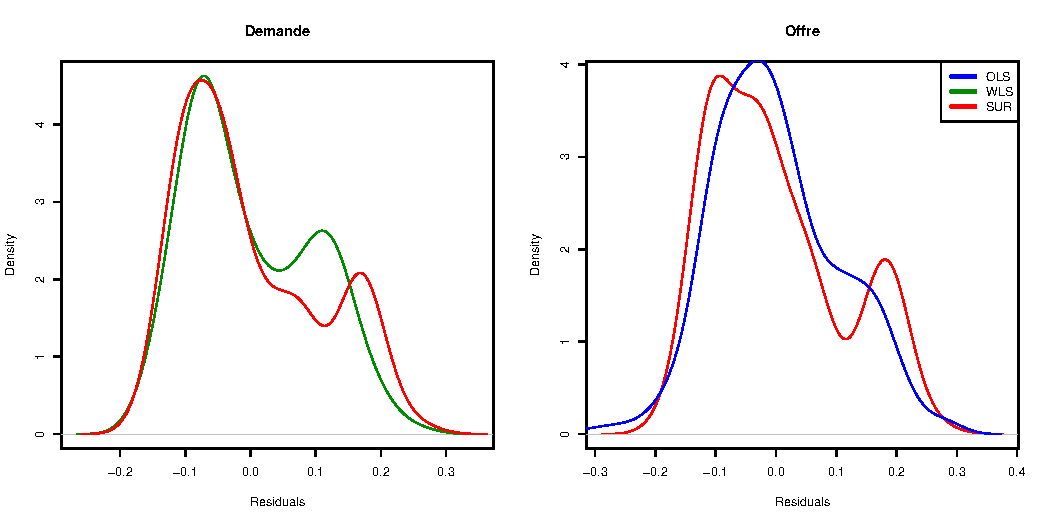
\includegraphics{note2pres_files/figure-latex/unnamed-chunk-47-1} 

}

\caption{Les PDF des résidus}\label{fig:unnamed-chunk-47}
\end{figure}

\FloatBarrier

\hypertarget{les-residus-contre-la-variable-predite}{%
\subsection{Les résidus contre la variable
prédite}\label{les-residus-contre-la-variable-predite}}

\FloatBarrier

\begin{figure}[!htbp]

{\centering 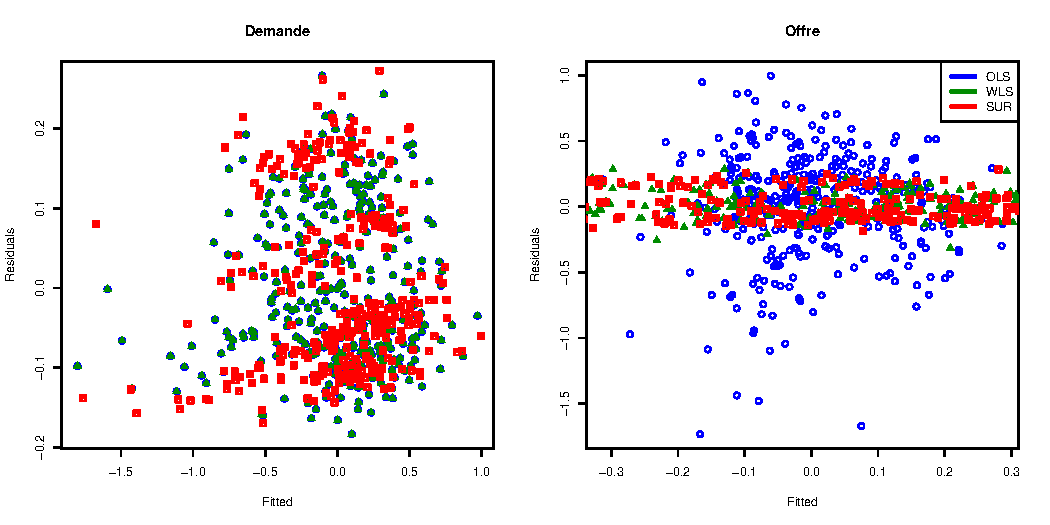
\includegraphics{note2pres_files/figure-latex/unnamed-chunk-48-1} 

}

\caption{Les résidus contre la variable prédite}\label{fig:unnamed-chunk-48}
\end{figure}

\FloatBarrier

\hypertarget{les-resultats-2sls-w2sls-3sls-et-i3sls}{%
\subsection{Les résultats 2SLS, W2SLS, 3SLS et
i3SLS}\label{les-resultats-2sls-w2sls-3sls-et-i3sls}}

\FloatBarrier

\FloatBarrier

\begin{table}[!htbp]
\begin{center}
\begin{tabular}{l c c c c }
\hline
 & 2SLS & W2SLS & 3SLS & i3SLS \\
\hline
Demande: ipi        & $1.19^{***}$  & $1.19^{***}$  & $1.19^{***}$  & $1.19^{***}$  \\
                    & $(0.06)$      & $(0.06)$      & $(0.06)$      & $(0.06)$      \\
Demande: ri         & $-5.67^{***}$ & $-5.67^{***}$ & $-5.67^{***}$ & $-5.67^{***}$ \\
                    & $(0.71)$      & $(0.71)$      & $(0.71)$      & $(0.71)$      \\
Offre: ipi          & $-1.22$       & $-1.22$       & $-0.71$       & $-0.81$       \\
                    & $(1.97)$      & $(1.97)$      & $(1.96)$      & $(1.60)$      \\
Offre: si           & $0.70$        & $0.70$        & $0.46$        & $0.51$        \\
                    & $(0.59)$      & $(0.59)$      & $(0.58)$      & $(0.47)$      \\
Offre: iki          & $-0.46$       & $-0.46$       & $-0.73^{*}$   & $-0.68^{*}$   \\
                    & $(0.34)$      & $(0.34)$      & $(0.32)$      & $(0.26)$      \\
\hline
Demande: R$^2$      & 0.88          & 0.88          & 0.88          & 0.88          \\
Offre: R$^2$        & -3.37         & -3.37         & -1.60         & -1.90         \\
Demande: Adj. R$^2$ & 0.88          & 0.88          & 0.88          & 0.88          \\
Offre: Adj. R$^2$   & -3.40         & -3.40         & -1.62         & -1.92         \\
Num. obs. (total)   & 690           & 690           & 690           & 690           \\
\hline
\multicolumn{5}{l}{\scriptsize{$^{***}p<0.001$, $^{**}p<0.01$, $^*p<0.05$}}
\end{tabular}
\caption{Statistical models}
\label{table : 2sls, w2sls, 3sls and fiml}
\end{center}
\end{table}

\FloatBarrier

\hypertarget{comparaison-des-modeles}{%
\subsection{Comparaison des modèles}\label{comparaison-des-modeles}}

\FloatBarrier

\FloatBarrier

\begin{table}[!htbp] \centering 
  \caption{Hausman 3SLS consistency test} 
  \label{} 
\begin{tabular}{@{\extracolsep{5pt}} ccc} 
\\[-1.8ex]\hline 
\hline \\[-1.8ex] 
 & Test & Resultats \\ 
\hline \\[-1.8ex] 
1 & 2SLS contre 3SLS & $0.350$ \\ 
2 & 2SLS contre i3SLS & $0.735$ \\ 
\hline \\[-1.8ex] 
\end{tabular} 
\end{table}

\FloatBarrier

\FloatBarrier

\FloatBarrier

\hypertarget{le-comportement-des-residus-1}{%
\subsection{Le comportement des
résidus}\label{le-comportement-des-residus-1}}

\FloatBarrier

\FloatBarrier

\begin{table}[!htbp] \centering 
  \caption{Shapiro-Wilk test de normalité} 
  \label{} 
\begin{tabular}{@{\extracolsep{5pt}} cccc} 
\\[-1.8ex]\hline 
\hline \\[-1.8ex] 
 & 2SLS & 3SLS & i3SLS \\ 
\hline \\[-1.8ex] 
Equation de demande & $0.00003$ & $0.00003$ & $0.00003$ \\ 
Equation d'offre & $0.00000$ & $0.00000$ & $0.00000$ \\ 
\hline \\[-1.8ex] 
\end{tabular} 
\end{table}

\FloatBarrier

\FloatBarrier

\FloatBarrier

\% Table created by stargazer v.5.2.2 by Marek Hlavac, Harvard
University. E-mail: hlavac at fas.harvard.edu \% Date and time: lun.,
déc. 16, 2019 - 13:26:38

\begin{table}[!htbp] \centering 
  \caption{Test de Bartlett sur l'heterockedacité} 
  \label{} 
\begin{tabular}{@{\extracolsep{5pt}} cccc} 
\\[-1.8ex]\hline 
\hline \\[-1.8ex] 
 & 2SLS & 3SLS & i3SLS \\ 
\hline \\[-1.8ex] 
Equation de demande & $0.975$ & $0.975$ & $0.975$ \\ 
Equation d'offre & $0.0003$ & $0.002$ & $0.001$ \\ 
\hline \\[-1.8ex] 
\end{tabular} 
\end{table}

\FloatBarrier

\hypertarget{les-pdf-des-residus-1}{%
\subsection{Les PDF des résidus}\label{les-pdf-des-residus-1}}

\FloatBarrier

\begin{figure}[!htbp]

{\centering 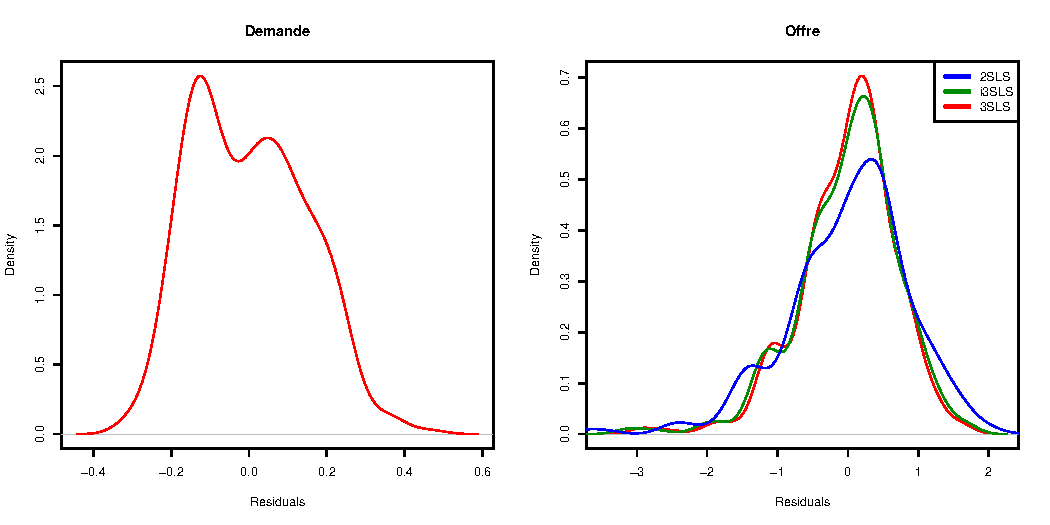
\includegraphics{note2pres_files/figure-latex/unnamed-chunk-60-1} 

}

\caption{Les PDF des résidus}\label{fig:unnamed-chunk-60}
\end{figure}

\FloatBarrier

\hypertarget{les-residus-contre-la-variable-predite-1}{%
\subsection{Les résidus contre la variable
prédite}\label{les-residus-contre-la-variable-predite-1}}

\FloatBarrier

\begin{figure}[!htbp]

{\centering 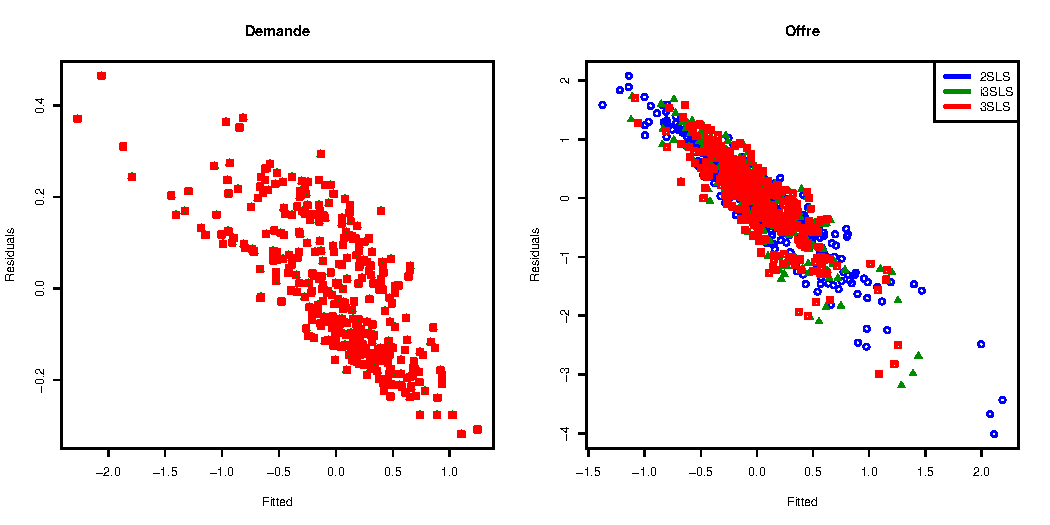
\includegraphics{note2pres_files/figure-latex/unnamed-chunk-61-1} 

}

\caption{Les résidus contre la variable prédite}\label{fig:unnamed-chunk-61}
\end{figure}

\FloatBarrier

\hypertarget{les-residus-et-les-predictions-pour-i3sls}{%
\subsection{Les résidus et les prédictions pour
i3SLS}\label{les-residus-et-les-predictions-pour-i3sls}}

\FloatBarrier

\begin{figure}[!htbp]

{\centering 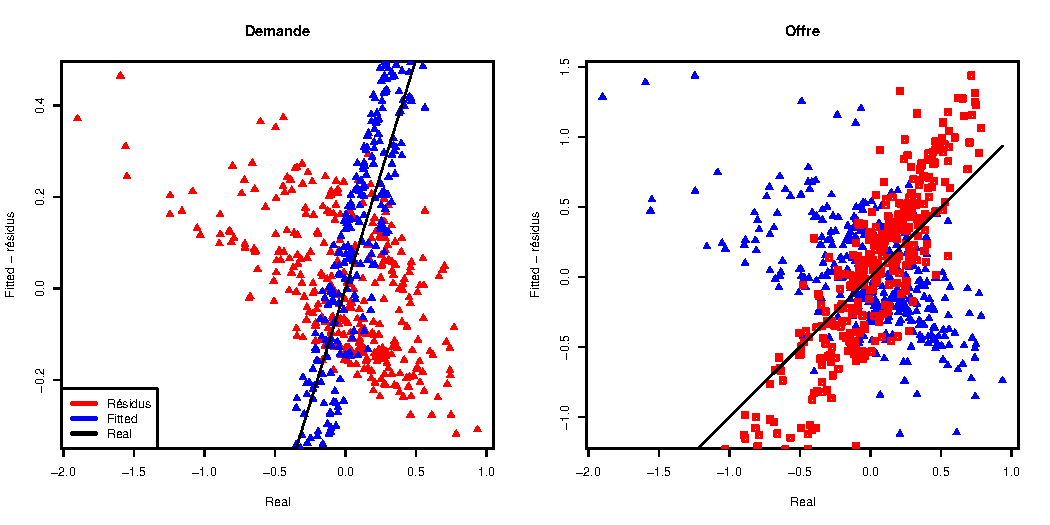
\includegraphics{note2pres_files/figure-latex/unnamed-chunk-62-1} 

}

\caption{Les résidus et les prédictions}\label{fig:unnamed-chunk-62}
\end{figure}

\FloatBarrier

\hypertarget{lautocorrelation}{%
\subsection{L'autocorrelation}\label{lautocorrelation}}

\FloatBarrier

\FloatBarrier

\FloatBarrier

\hypertarget{lautocorrelation-sur-2-dimentions-pour-i3sls}{%
\subsection{L'autocorrelation sur 2 dimentions pour
i3SLS}\label{lautocorrelation-sur-2-dimentions-pour-i3sls}}

\FloatBarrier

\begin{figure}[!htbp]

{\centering 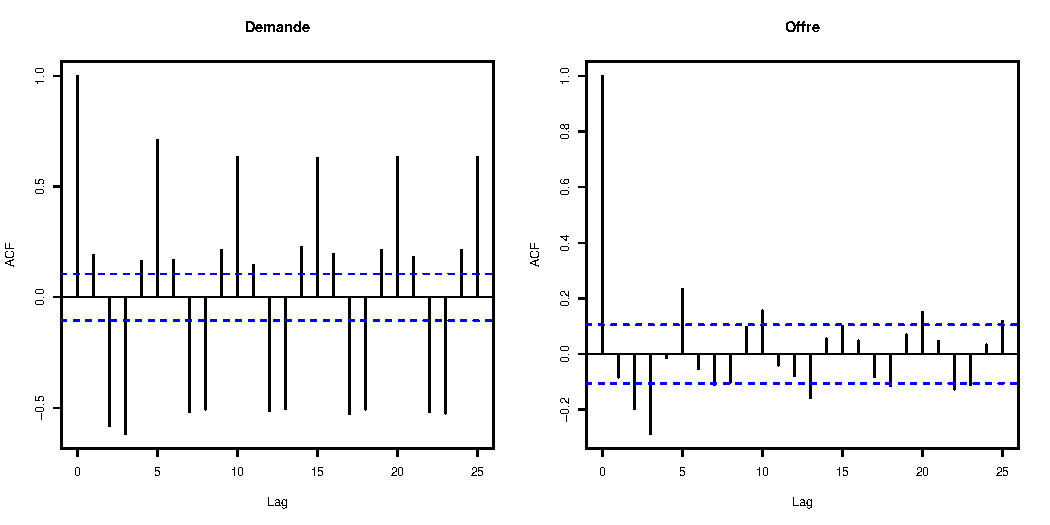
\includegraphics{note2pres_files/figure-latex/unnamed-chunk-65-1} 

}

\caption{L'autocorrelation pour le modèle  i3SLS}\label{fig:unnamed-chunk-65}
\end{figure}

\FloatBarrier

\hypertarget{lindependance-des-residus}{%
\subsection{L'independance des
résidus}\label{lindependance-des-residus}}

\FloatBarrier

\FloatBarrier

\FloatBarrier

\hypertarget{clustering-et-la-separation-des-groupes-between-transformation-approach}{%
\section{Clustering et la séparation des groupes (Between transformation
approach)}\label{clustering-et-la-separation-des-groupes-between-transformation-approach}}

Nous avons vus dans le comportement des résidus une nature non-aléatoire
grouppé. Cela nous amène à l'idée de construire k-clusters pour
modèliser les rélations par grouppe.

\par

Nous supposons que les départements ayant des valeurs moyennes
interannuelles proches (transformation Between) ont le comportement
identique. La clusterisation est effectué sur les données Between pour
les départements.

\par

Nous povons supposer que le nombre des clusters optimal est entre 3 et
5. Prenant en compte les graphiques des résidus vus lros d'analse des
modèles nous allons supposer qu'il n'y a que 3 clusters principaux.

\FloatBarrier

\begin{figure}[!htbp]

{\centering 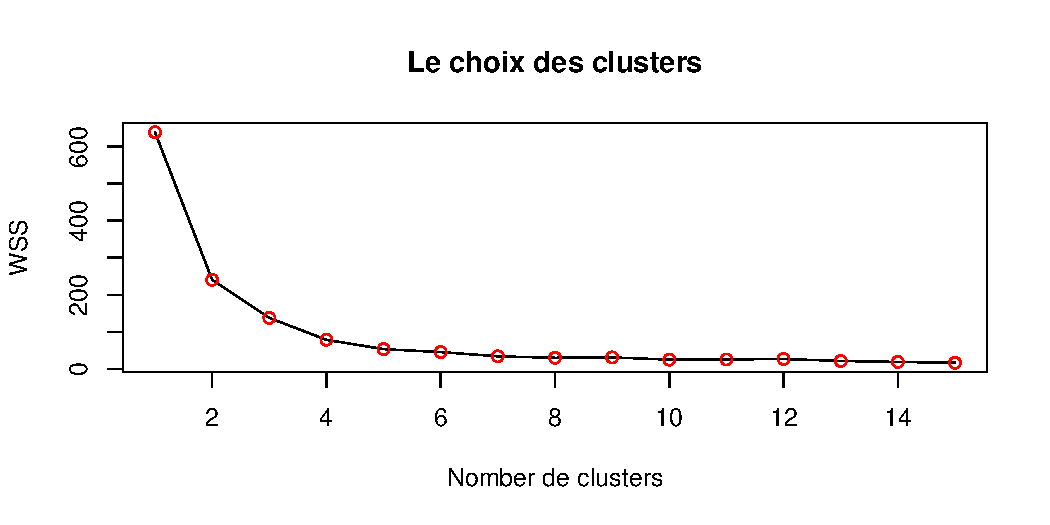
\includegraphics{note2pres_files/figure-latex/unnamed-chunk-69-1} 

}

\caption{Le choix des clusters}\label{fig:unnamed-chunk-69}
\end{figure}

\FloatBarrier

Les groupes sont définies par des caractéristiques suivantes :

\FloatBarrier

\begin{table}[!htbp] \centering 
  \caption{Les centres des clusters} 
  \label{} 
\begin{tabular}{@{\extracolsep{5pt}} ccccccc} 
\\[-1.8ex]\hline 
\hline \\[-1.8ex] 
 & qi & ipi & si & ri & iki & .1 \\ 
\hline \\[-1.8ex] 
1 & $5.349$ & $0.190$ & $2.311$ & $9.880$ & $0.216$ & $17$ \\ 
2 & $8.207$ & $0.154$ & $4.879$ & $9.914$ & $0.136$ & $31$ \\ 
3 & $10.940$ & $0.192$ & $7.000$ & $9.867$ & $0.184$ & $21$ \\ 
\hline \\[-1.8ex] 
\end{tabular} 
\end{table}

\FloatBarrier

\hypertarget{modelisation-1}{%
\subsection{Modèlisation}\label{modelisation-1}}

\FloatBarrier

Nous evaluons le système en introduisant les variables de grouppe (dummy
variables) sous l'hypothèse des résidus joints.

\FloatBarrier

\FloatBarrier

\begin{table}[!htbp]
\begin{center}
\begin{tabular}{l c c c }
\hline
 & OLS & 2SLS & 3SLS \\
\hline
Demande: ipi        & $0.93^{***}$  & $1.14^{***}$  & $1.13^{***}$  \\
                    & $(0.01)$      & $(0.05)$      & $(0.05)$      \\
Demande: ri1        & $-5.42^{***}$ & $-4.20^{**}$  & $-5.64^{***}$ \\
                    & $(0.94)$      & $(1.30)$      & $(1.21)$      \\
Demande: ri2        & $-6.58^{***}$ & $-7.21^{***}$ & $-7.69^{***}$ \\
                    & $(0.68)$      & $(0.93)$      & $(0.91)$      \\
Demande: ri3        & $-4.54^{***}$ & $-4.30^{***}$ & $-4.21^{***}$ \\
                    & $(0.92)$      & $(1.25)$      & $(1.19)$      \\
Offre: ipi          & $0.89^{***}$  & $0.41^{*}$    & $0.41^{*}$    \\
                    & $(0.01)$      & $(0.20)$      & $(0.20)$      \\
Offre: si1          & $0.05^{**}$   & $0.19^{**}$   & $0.18^{*}$    \\
                    & $(0.02)$      & $(0.07)$      & $(0.07)$      \\
Offre: si2          & $0.09^{***}$  & $0.20^{**}$   & $0.21^{**}$   \\
                    & $(0.02)$      & $(0.06)$      & $(0.06)$      \\
Offre: si3          & $0.30^{***}$  & $0.74^{**}$   & $0.72^{**}$   \\
                    & $(0.06)$      & $(0.23)$      & $(0.22)$      \\
Offre: iki1         & $-0.22^{***}$ & $-0.26^{*}$   & $-0.36^{***}$ \\
                    & $(0.05)$      & $(0.11)$      & $(0.10)$      \\
Offre: iki2         & $-0.18^{***}$ & $-0.34^{**}$  & $-0.34^{***}$ \\
                    & $(0.04)$      & $(0.10)$      & $(0.10)$      \\
Offre: iki3         & $-0.09^{*}$   & $0.03$        & $-0.06$       \\
                    & $(0.04)$      & $(0.11)$      & $(0.10)$      \\
\hline
Demande: R$^2$      & 0.95          & 0.90          & 0.90          \\
Offre: R$^2$        & 0.94          & 0.72          & 0.73          \\
Demande: Adj. R$^2$ & 0.95          & 0.90          & 0.90          \\
Offre: Adj. R$^2$   & 0.94          & 0.72          & 0.72          \\
Num. obs. (total)   & 690           & 690           & 690           \\
\hline
\multicolumn{4}{l}{\scriptsize{$^{***}p<0.001$, $^{**}p<0.01$, $^*p<0.05$}}
\end{tabular}
\caption{Statistical models}
\label{table : ols, 2sls et 3sls}
\end{center}
\end{table}

\FloatBarrier

\hypertarget{tests}{%
\subsection{Tests}\label{tests}}

Etudions la validité du modèle 3SLS :

\FloatBarrier

\FloatBarrier

\begin{table}[!htbp] \centering 
  \caption{Hausman 3SLS consistency test} 
  \label{} 
\begin{tabular}{@{\extracolsep{5pt}} ccc} 
\\[-1.8ex]\hline 
\hline \\[-1.8ex] 
 & Test & Resultats \\ 
\hline \\[-1.8ex] 
1 & 2SLS contre 3SLS & $0$ \\ 
\hline \\[-1.8ex] 
\end{tabular} 
\end{table}

La normalité des résidus :

\FloatBarrier

\begin{table}[!htbp] \centering 
  \caption{Shapiro-Wilk normality test} 
  \label{} 
\begin{tabular}{@{\extracolsep{5pt}} cccc} 
\\[-1.8ex]\hline 
\hline \\[-1.8ex] 
 & OLS & 2SLS & 3SLS \\ 
\hline \\[-1.8ex] 
Equation de demande & $0$ & $0.00001$ & $0.00001$ \\ 
Equation d'offre & $0.001$ & $0$ & $0$ \\ 
\hline \\[-1.8ex] 
\end{tabular} 
\end{table}

\FloatBarrier

L'heteroscedacité :

\FloatBarrier

\FloatBarrier

\begin{table}[!htbp] \centering 
  \caption{Bartlett heteroscedasticity test} 
  \label{} 
\begin{tabular}{@{\extracolsep{5pt}} cccc} 
\\[-1.8ex]\hline 
\hline \\[-1.8ex] 
 & OLS & 2SLS & 3SLS \\ 
\hline \\[-1.8ex] 
Equation de demande & $0.977$ & $0.987$ & $0.974$ \\ 
Equation d'offre & $0.989$ & $0.00000$ & $0.00000$ \\ 
\hline \\[-1.8ex] 
\end{tabular} 
\end{table}

\FloatBarrier

Les PDF des résidus :

\FloatBarrier

\begin{center}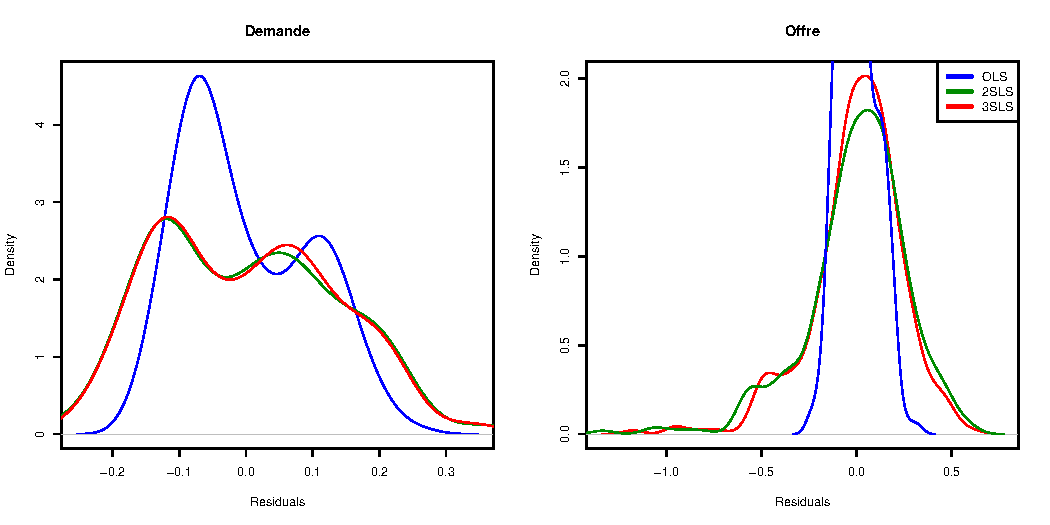
\includegraphics{note2pres_files/figure-latex/unnamed-chunk-82-1} \end{center}

\FloatBarrier

Les résidus contre les variables prédites :

\FloatBarrier

\begin{center}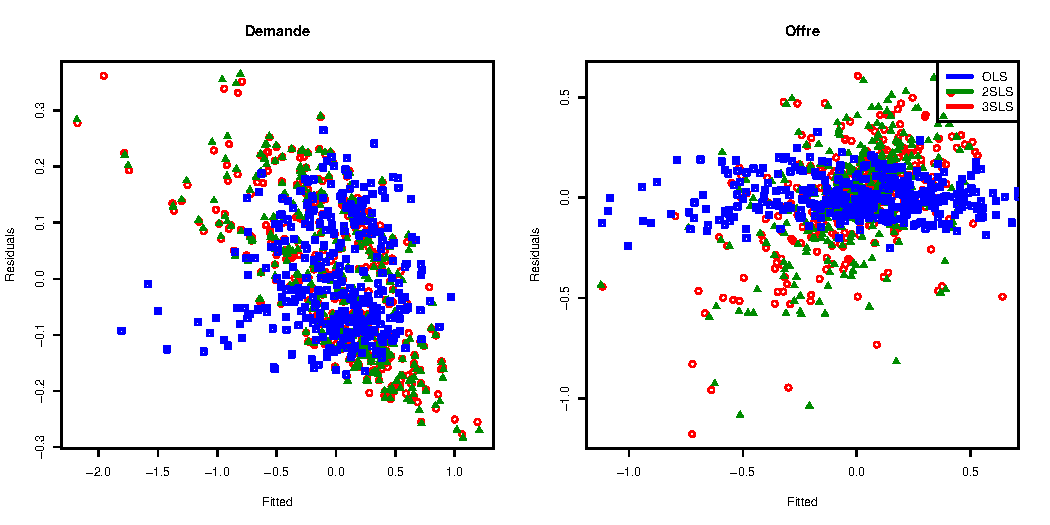
\includegraphics{note2pres_files/figure-latex/unnamed-chunk-83-1} \end{center}

Conclusion : les problèmes restent non résolus.

\FloatBarrier

\hypertarget{clustering-et-la-separation-des-groupes-wide-data-approach}{%
\section{Clustering et la séparation des groupes (WIDE data
approach)}\label{clustering-et-la-separation-des-groupes-wide-data-approach}}

Nous avons vus dans le comportement des résidus une nature non-aléatoire
grouppé. Cela nous amène à l'idée de construire k-clusters pour
modèliser les rélations par grouppe.

\par

D'abord on compare le comportement des cluster pour les données à
l'information complete et les données Within.

\hypertarget{transformation-within}{%
\subsection{Transformation Within}\label{transformation-within}}

Comme nous pouvons voir dans les résultats le nombre des cluster
optimaux est trop large pour les séparer dans l'analyse :

\par

Nous povons supposer que le nombre des clusters optimal est entre 6 et
15.

\FloatBarrier

\begin{center}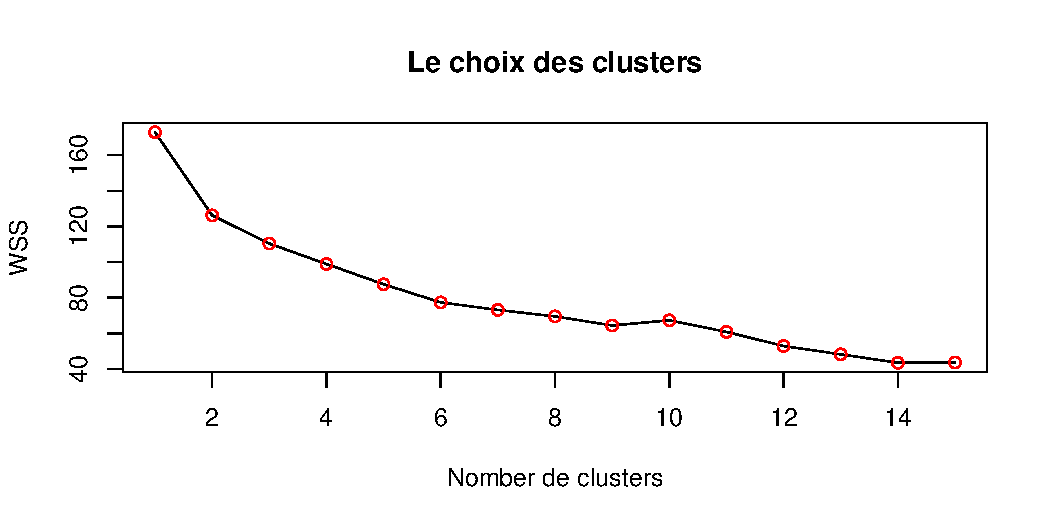
\includegraphics{note2pres_files/figure-latex/unnamed-chunk-87-1} \end{center}

\FloatBarrier

Les groupes sont définies par des caractéristiques suivantes :

\FloatBarrier

Representation graphique :

\begin{center}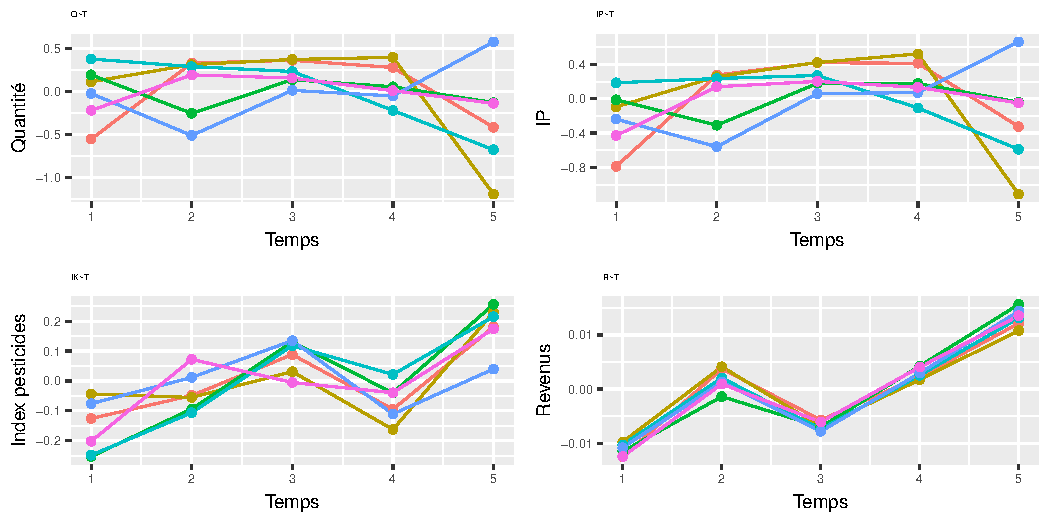
\includegraphics{note2pres_files/figure-latex/unnamed-chunk-90-1} \end{center}

\hypertarget{information-complete}{%
\subsection{Information complete}\label{information-complete}}

Dans le cas d'information complete on a :

\par

Nous povons supposer que le nombre des clusters optimal est entre 3 et
5. Prenant en compte les graphiques des résidus vus lros d'analse des
modèles nous allons supposer qu'il n'y a que 3 clusters principaux.

\FloatBarrier

\begin{center}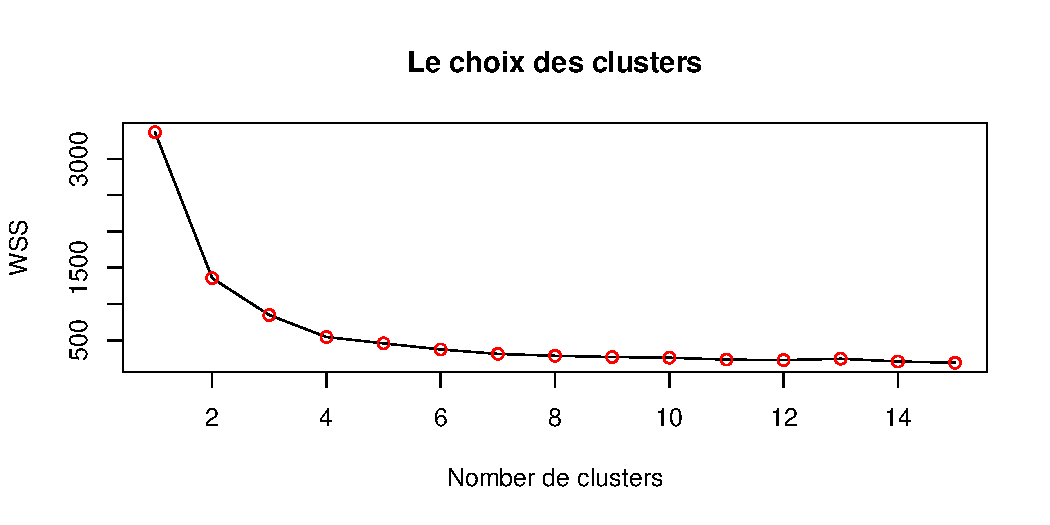
\includegraphics{note2pres_files/figure-latex/unnamed-chunk-94-1} \end{center}

\FloatBarrier

Les groupes sont définies par des caractéristiques suivantes :

\FloatBarrier

\begin{table}[!htbp] \centering 
  \caption{Les centres des clusters} 
  \label{} 
\begin{tabular}{@{\extracolsep{5pt}} ccccccccc} 
\\[-1.8ex]\hline 
\hline \\[-1.8ex] 
 & qi & ipi & si & ri & iki & n & k & t \\ 
\hline \\[-1.8ex] 
1 & 10.905002 & 0 & 7.048328 & 9.860348 & 0 & 22 & 1 & 1 \\ 
2 & 10.691657 & -0.056005 & 6.945538 & 9.872895 & 0.149462 & 22 & 1 & 2 \\ 
3 & 10.990015 & 0.338205 & 6.984754 & 9.859395 & 0.302499 & 22 & 1 & 3 \\ 
4 & 10.952753 & 0.380444 & 6.855669 & 9.87067 & 0.100718 & 22 & 1 & 4 \\ 
5 & 10.906341 & 0.294342 & 6.830466 & 9.881679 & 0.36276 & 22 & 1 & 5 \\ 
6 & 8.204277 & 0 & 4.987838 & 9.900816 & 0 & 30 & 2 & 1 \\ 
7 & 8.175461 & 0.122615 & 5.007068 & 9.913384 & 0.10792 & 30 & 2 & 2 \\ 
8 & 8.360791 & 0.406721 & 4.908536 & 9.909318 & 0.153133 & 30 & 2 & 3 \\ 
9 & 8.161618 & 0.281943 & 4.746188 & 9.919147 & 0.087094 & 30 & 2 & 4 \\ 
10 & 7.864193 & -0.044913 & 4.637459 & 9.929119 & 0.326554 & 30 & 2 & 5 \\ 
11 & 5.37234 & 0 & 2.473289 & 9.869431 & 0 & 17 & 3 & 1 \\ 
12 & 5.61569 & 0.404064 & 2.55531 & 9.881971 & 0.158519 & 17 & 3 & 2 \\ 
13 & 5.619106 & 0.509682 & 2.302302 & 9.872995 & 0.376623 & 17 & 3 & 3 \\ 
14 & 5.448956 & 0.419102 & 2.217837 & 9.881977 & 0.147986 & 17 & 3 & 4 \\ 
15 & 4.689674 & -0.381999 & 2.008663 & 9.892485 & 0.399327 & 17 & 3 & 5 \\ 
\hline \\[-1.8ex] 
\end{tabular} 
\end{table}

Representation graphique :

\begin{center}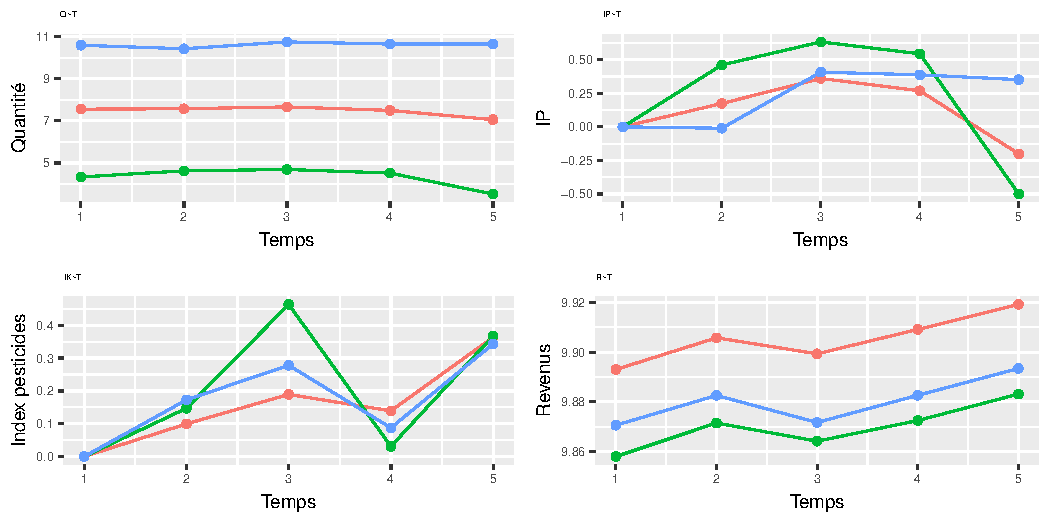
\includegraphics{note2pres_files/figure-latex/unnamed-chunk-97-1} \end{center}

\FloatBarrier

\hypertarget{modelisation-2}{%
\subsection{Modèlisation}\label{modelisation-2}}

\FloatBarrier

Nous evaluons le système en introduisant les variables de grouppe (dummy
variables) sous l'hypothèse des résidus joints.

\FloatBarrier

\FloatBarrier

\hypertarget{tests-1}{%
\subsection{Tests}\label{tests-1}}

\FloatBarrier

\begin{table}[!htbp]
\begin{center}
\begin{tabular}{l c c c }
\hline
 & OLS & 2SLS & 3SLS \\
\hline
Demande: ipi        & $0.93^{***}$  & $1.14^{***}$  & $1.14^{***}$  \\
                    & $(0.01)$      & $(0.05)$      & $(0.05)$      \\
Demande: ri1        & $-4.63^{***}$ & $-4.64^{***}$ & $-4.49^{***}$ \\
                    & $(0.91)$      & $(1.24)$      & $(1.19)$      \\
Demande: ri2        & $-6.56^{***}$ & $-7.07^{***}$ & $-7.66^{***}$ \\
                    & $(0.69)$      & $(0.94)$      & $(0.91)$      \\
Demande: ri3        & $-5.43^{***}$ & $-4.18^{**}$  & $-5.65^{***}$ \\
                    & $(0.94)$      & $(1.31)$      & $(1.22)$      \\
Offre: ipi          & $0.89^{***}$  & $0.42^{*}$    & $0.43^{*}$    \\
                    & $(0.01)$      & $(0.20)$      & $(0.20)$      \\
Offre: si1          & $0.30^{***}$  & $0.74^{**}$   & $0.72^{**}$   \\
                    & $(0.06)$      & $(0.23)$      & $(0.22)$      \\
Offre: si2          & $0.09^{***}$  & $0.19^{**}$   & $0.19^{**}$   \\
                    & $(0.02)$      & $(0.06)$      & $(0.06)$      \\
Offre: si3          & $0.05^{**}$   & $0.19^{**}$   & $0.17^{*}$    \\
                    & $(0.02)$      & $(0.07)$      & $(0.07)$      \\
Offre: iki1         & $-0.09^{*}$   & $0.02$        & $-0.07$       \\
                    & $(0.04)$      & $(0.11)$      & $(0.10)$      \\
Offre: iki2         & $-0.18^{***}$ & $-0.33^{**}$  & $-0.33^{**}$  \\
                    & $(0.04)$      & $(0.10)$      & $(0.10)$      \\
Offre: iki3         & $-0.22^{***}$ & $-0.26^{*}$   & $-0.35^{***}$ \\
                    & $(0.05)$      & $(0.11)$      & $(0.10)$      \\
\hline
Demande: R$^2$      & 0.95          & 0.90          & 0.90          \\
Offre: R$^2$        & 0.94          & 0.73          & 0.74          \\
Demande: Adj. R$^2$ & 0.95          & 0.90          & 0.90          \\
Offre: Adj. R$^2$   & 0.94          & 0.73          & 0.74          \\
Num. obs. (total)   & 690           & 690           & 690           \\
\hline
\multicolumn{4}{l}{\scriptsize{$^{***}p<0.001$, $^{**}p<0.01$, $^*p<0.05$}}
\end{tabular}
\caption{Statistical models}
\label{table : ols, 2sls et 3sls, full information clusters}
\end{center}
\end{table}

\FloatBarrier

Etudions la validité du modèle 3SLS :

\FloatBarrier

\FloatBarrier

\begin{table}[!htbp] \centering 
  \caption{Hausman 3SLS consistency test} 
  \label{} 
\begin{tabular}{@{\extracolsep{5pt}} ccc} 
\\[-1.8ex]\hline 
\hline \\[-1.8ex] 
 & Test & Resultats \\ 
\hline \\[-1.8ex] 
1 & 2SLS contre 3SLS & $0.0003$ \\ 
\hline \\[-1.8ex] 
\end{tabular} 
\end{table}

La normalité des résidus :

\FloatBarrier

\begin{table}[!htbp] \centering 
  \caption{Shapiro-Wilk normality test} 
  \label{} 
\begin{tabular}{@{\extracolsep{5pt}} cccc} 
\\[-1.8ex]\hline 
\hline \\[-1.8ex] 
 & OLS & 2SLS & 3SLS \\ 
\hline \\[-1.8ex] 
Equation de demande & $0$ & $0.00001$ & $0.00001$ \\ 
Equation d'offre & $0.001$ & $0$ & $0$ \\ 
\hline \\[-1.8ex] 
\end{tabular} 
\end{table}

\FloatBarrier

L'heteroscedacité :

\FloatBarrier

\FloatBarrier

\begin{table}[!htbp] \centering 
  \caption{Bartlett heteroscedasticity test} 
  \label{} 
\begin{tabular}{@{\extracolsep{5pt}} cccc} 
\\[-1.8ex]\hline 
\hline \\[-1.8ex] 
 & OLS & 2SLS & 3SLS \\ 
\hline \\[-1.8ex] 
Equation de demande & $0.975$ & $0.985$ & $0.969$ \\ 
Equation d'offre & $0.989$ & $0.00000$ & $0.00000$ \\ 
\hline \\[-1.8ex] 
\end{tabular} 
\end{table}

\FloatBarrier

Les PDF des résidus :

\FloatBarrier

\begin{center}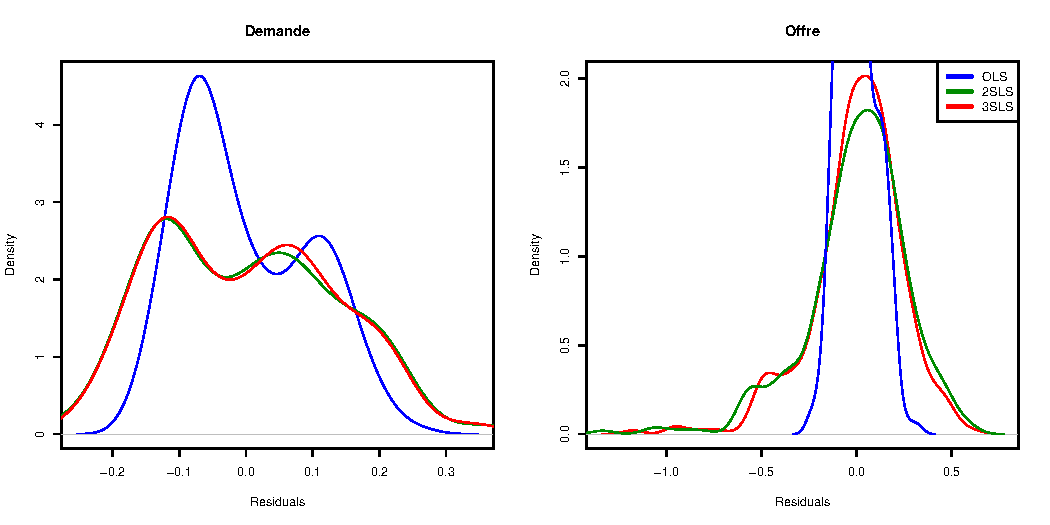
\includegraphics{note2pres_files/figure-latex/unnamed-chunk-108-1} \end{center}

\FloatBarrier

Les résidus contre les variables prédites :

\FloatBarrier

\begin{center}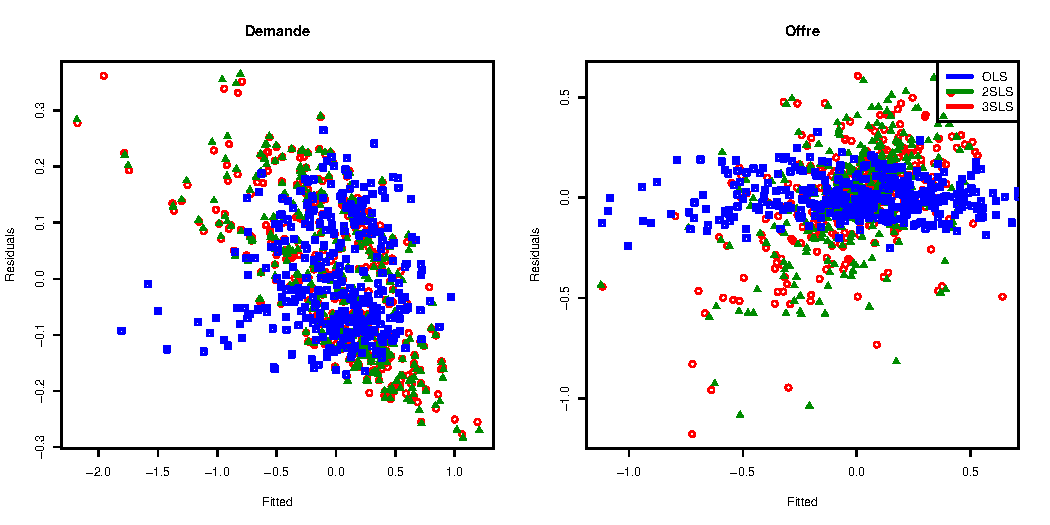
\includegraphics{note2pres_files/figure-latex/unnamed-chunk-109-1} \end{center}

Conclusion : les problèmes restent non résolus.

\FloatBarrier

\hypertarget{conclusions}{%
\section{Conclusions}\label{conclusions}}

\FloatBarrier

\FloatBarrier

\hypertarget{conclusions-1}{%
\subsection{Conclusions}\label{conclusions-1}}

\begin{itemize}
\tightlist
\item
  Le marché du vin
\item
  Le rôle des pésticides\\
\item
  Validité
\end{itemize}

\FloatBarrier

\hypertarget{le-marche-du-vin}{%
\subsection{Le marché du vin}\label{le-marche-du-vin}}

\begin{itemize}
\tightlist
\item
  Un comportement inattendus

  \begin{itemize}
  \item
    Les effets de substitution contre les produits de la haute gamme
  \item
    Les effets négatives du revenu
  \item
  \end{itemize}
\end{itemize}

\FloatBarrier

\hypertarget{le-role-des-pesticides}{%
\subsection{Le rôle des pésticides}\label{le-role-des-pesticides}}

\begin{itemize}
\tightlist
\item
  Confirmation des résultats des études précedentes

  \begin{itemize}
  \tightlist
  \item
    Utilisés pour réduire les pertes
  \end{itemize}
\end{itemize}

\FloatBarrier

\hypertarget{validite}{%
\subsection{Validité}\label{validite}}

\begin{itemize}
\tightlist
\item
  Faible validité du modèle économétrique

  \begin{itemize}
  \tightlist
  \item
    Variables ommises
  \end{itemize}
\end{itemize}

\FloatBarrier

\begin{itemize}
\tightlist
\item
  Cembalo L., Caracciolo F., \& Pomarici E. (2014). ``Drinking cheaply :
  the demand for basic wine in italy.'' \emph{Australian Journal of
  Agricultural and Resource Economics}, 58(3). 374-391.
\item
  Butault J-P., Delame N., Jacquet F. \& Zardet G. (2011).
  ``L'utilisation des pesticides en France: état des lieux et
  perspectives de réduction.'' \emph{Notes et études socio-économiques},
  35. 7-26
\item
  Pujol J. (2017). ``Apports des produits phytosanitaires en viticulture
  et climat : une analyse à partir des enquêtes pratiques culturales.''
  \emph{Agreste Les Dossiers}. 39. 3-25
\end{itemize}

Cembalo, Caracciolo, and Pomarici (2014)

\hypertarget{references}{%
\section*{References}\label{references}}
\addcontentsline{toc}{section}{References}

\hypertarget{refs}{}
\leavevmode\hypertarget{ref-cembalo2014}{}%
Cembalo, Luigi, Francesco Caracciolo, and Eugenio Pomarici. 2014.
``Drinking Cheaply: The Demand for Basic Wine in Italy.''
\emph{Australian Journal of Agricultural and Resource Economics} 58 (3):
374--91.


\end{document}
